\documentclass[a4paper,twoside,11pt,
                %draft,%
              ]{scrbook} 
\usepackage[top=2.5cm,bottom=3.0cm,inner=3.0cm,outer=3.0cm]{geometry}

\usepackage{ifdraft}
\usepackage{ifthen}
\usepackage{amsmath}

%%%%%%%%%%%%%%%%%%%%%%%%%%%%%%%%%%%%%%%%
%\includeonly{abstract,tub-eidesstattliche}
%%%%%%%%%%%%%%%%%%%%%%%%%%%%%%%%%%%%%%%%

%%%% common header file for final and draft mode
\usepackage[utf8]{inputenc}
\usepackage[T1]{fontenc}
%\usepackage{lmodern}
\usepackage[ngerman,UKenglish]{babel}
\usepackage[protrusion, expansion]{microtype}
\usepackage{textcomp}
\usepackage{xspace}
\usepackage[dvipsnames,svgnames]{xcolor}
\usepackage{floatrow}
\DeclareColorBox{imgbg}{\fcolorbox{white}{white}}

\ifdraft{%
    \linespread{1.25}  % Zeilenabstand fuer Korrekturen

\usepackage{geometry}
\geometry{includehead, includefoot, 
    left=30mm,right=25mm, top= 10mm, bottom= 10mm}
\setboolean{@twoside}{false} % einseitiges Layout

\usepackage[missing={Help-missing!}]{gitinfo}

\usepackage{fancyhdr}
\pagestyle{fancy}

%%%% floatrow options
%\floatsetup{capposition=top}
\floatsetup[widefigure]{capposition=bottom,floatwidth=\textwidth}
\floatsetup[table]{capposition=top}

%\usepackage[]{caption}
%\captionsetup{labelfont=bf,font={sf,footnotesize},format=plain,labelsep=period}

\lhead{\rightmark}
\rhead{(\the\day.\the\month.\the\year)~~~-\thepage-}
\lfoot{\footnotesize \emph{Git revision\gitVtags:} \parbox[t]{.60\textwidth}{\gitAuthorIsoDate~\gitReferences}}
\cfoot{}
\rfoot{\footnotesize \emph{Git abbrev. hash}: {\ttfamily\gitAbbrevHash}}
\renewcommand{\footrulewidth}{0.4pt}
\renewcommand{\headrulewidth}{0pt}


}{%
    %%%% Textsatz, Layout, Stil
\usepackage[osf]{mathpazo} % auch Palatino, andere math font
\linespread{1.05}         % Palatino needs more leading (space between lines)
%\usepackage[scaled=0.86]{berasans} % serifenlose Schrift
%\usepackage[scaled]{helvet} serifenlose Schrift
\usepackage[defaultsans]{droidsans} % serifenlose Schrift -- DIE HIER wäre schick!
\usepackage[scaled=1.03]{inconsolata}

%Überschriften serifenlos und über den Rand hängend
\usepackage[sf,sl,outermarks,noindentafter,nobottomtitles]{titlesec}

%könnte alles auch mit \bfseries versehen werden nach Geschmack
\titleformat{\section}[hang]{\LARGE\sffamily}{\thetitle}{8pt}{}
\titleformat{\subsection}[hang]{\Large\sffamily}{\thetitle}{8pt}{}
\titleformat{\subsubsection}[hang]{\large\sffamily}{\thetitle}{8pt}{}
\titleformat{\paragraph}[hang]{\bfseries\sffamily}{\thetitle}{8pt}{}
%Etwas aufwendiger für die Kapitelüberschriften:
\titleformat{\chapter}[display]
{\filleft\Huge\sffamily} %Huge ist die Größe für Titeltext und Nummer
{\fontsize{100pt}{90pt}\selectfont\thechapter}
{-2ex} %is vertical space in [display] mode
%Platz vor dem ganzen Krempel
{\vspace{1ex}}
%Platz danach
[\vspace{1ex}]

%%% TOC design
\usepackage[titles]{tocloft}
\setlength{\cftbeforechapskip}{1ex}
\setlength{\cftbeforesecskip}{0.8ex}
\setlength{\cftbeforesubsecskip}{0.8ex}

%\renewcommand{\cftchapfont}{\sffamily\bfseries}
%\renewcommand{\cftchappagefont}{\sffamily}
%\renewcommand{\cftsecfont}{\sffamily}
%\renewcommand{\cftsecpagefont}{\sffamily}
%\renewcommand{\cftsubsecfont}{\sffamily}
%\renewcommand{\cftsubsecpagefont}{\sffamily}

\renewcommand{\cftpnumalign}{l}
\renewcommand{\cftsecdotsep}{\cftnodots}
\renewcommand{\cftsubsecdotsep}{\cftnodots}
\renewcommand{\cftchapleader}{\hspace{2em}}
\renewcommand{\cftsecleader}{\hspace{2em}}
\renewcommand{\cftsubsecleader}{\hspace{2em}}
\renewcommand{\cftchapafterpnum}{\cftparfillskip}
\renewcommand{\cftsecafterpnum}{\cftparfillskip}
\renewcommand{\cftsubsecafterpnum}{\cftparfillskip}

%%%% Grafiken, Abbildungen
\floatsetup{
    capposition=beside,
    capbesideposition={top,outside},
    facing=yes,
    floatwidth=.75\linewidth,
    capbesidewidth=sidefil,
    capbesidesep=quad,
    floatrowsep=quad,
    %framestyle=colorbox,framearound=all,colorframeset=imgbg,frameset={\fboxrule0pt},
    }
\floatsetup[widefigure]{%
    floatwidth=0.95\textwidth,
    %margins=hangoutside,
    %capposition=beside,
    capposition=below,
    %capbesideposition={top,outside},
    %capbesidewidth=\marginparwidth,
    %capbesideframe=yes,
    %capbesidesep=columnsep,
    %floatrowsep=columnsep,
    %heightadjust=nocaption,
    facing=yes,
    }
\floatsetup[widetable]{%
    floatwidth=0.95\textwidth,
    %margins=hangoutside,
    %capposition=beside,
    capposition=above,
    %capbesideposition={top,outside},
    %capbesidewidth=\marginparwidth,
    %capbesideframe=yes,
    %capbesidesep=columnsep,
    %floatrowsep=columnsep,
    %heightadjust=nocaption,
    facing=yes,
    }
\floatsetup[widefloat]{%
    floatwidth=0.95\textwidth,
    %margins=hangoutside,
    %capposition=beside,
    capposition=below,
    %capbesideposition={top,outside},
    %capbesidewidth=\marginparwidth,
    %capbesideframe=yes,
    %capbesidesep=columnsep,
    %floatrowsep=columnsep,
    %heightadjust=nocaption,
    facing=yes,
    }
\usepackage[]{caption}
\DeclareCaptionLabelSeparator{vbar}{ | } % custom; standard z.B. colon, period, ...
\captionsetup{labelfont=bf,font={sf,footnotesize},format=plain,labelsep=vbar}


}

%%%%% Bibliografie
\usepackage[autostyle,english=british,autopunct]{csquotes}
\usepackage[backend=biber,sorting=nyt,
            %style=authoryear-comp,autocite=footnote,
            style=numeric-comp,autocite=plain,
            firstinits=true,uniquename=init,backref=false,
            maxbibnames=25,minbibnames=10,maxcitenames=2,
            url=false,doi=true,isbn=false,eprint=true,
            ]{biblatex}

\addbibresource{zotero-full.bib}

%%% fine-tuning of the appearance
\AtEveryBibitem{\clearfield{month}}
\AtEveryBibitem{\clearfield{day}}
\renewcommand{\labelnamepunct}{\addcolon\addspace}
\DeclareFieldFormat[article]{volume}{\mkbibbold{#1}}
\DeclareCiteCommand{\citepatent}
    [\mkbibfootnote]
    {\usebibmacro{prenote}}
    {patent \printtext[bibhyperref]{\thefield{number}}}
    {\multicitedelim}
    {\usebibmacro{postnote}}
\DeclareCiteCommand{\supercite}
    [\mkbibsuperscript]
    {%
        \usebibmacro{cite:init}%
        \let\multicitedelim=\supercitedelim
        \iffieldundef{prenote}
        {}
        {\BibliographyWarning{Ignoring prenote argument}}%
        \iffieldundef{postnote}
        {}
        {\BibliographyWarning{Ignoring postnote argument}}%
        \bibopenbracket
    }%
    {\usebibmacro{citeindex}%
    \usebibmacro{cite:comp}}
    {}
    {\usebibmacro{cite:dump}\bibclosebracket}

\DeclareCiteCommand{\mycite}
    []
    {\usebibmacro{prenote}}
    {%
        \printnames[][-\value{listtotal}]{author}: %
        \printfield{title}, %
        \iffieldundef{booktitle}
            {\printfield{journaltitle} }
            {\printfield{booktitle} }
        \printfield{volume}.\printfield{number} (\printfield{year}), %
        \printfield{pages}%
    }
    {\multicitedelim}
    {\usebibmacro{postnote}}

%\DeclareCiteCommand{\publistcite}
    %[]
    %{\usebibmacro{prenote}}
    %{%
        %\printnames[][-\value{listtotal}]{author}: %
        %\printfield{title}, %
        %\printfield{journaltitle} \printfield{volume}.\printfield{number} (\printfield{year}), %
        %\printfield{pages}%
        %\printfield{doi}%
    %}
    %{\multicitedelim}
    %{\usebibmacro{postnote}}

\makeatletter
%%%% use maxbibnames instead of maxcitenames in fullcite:
\DeclareCiteCommand{\fullcite}
  {\defcounter{maxnames}{\blx@maxbibnames}%
    \usebibmacro{prenote}}
  {\usedriver
     {\DeclareNameAlias{sortname}{default}}
     {\thefield{entrytype}}}
  {\multicitedelim}
  {\usebibmacro{postnote}}
\makeatother

\let\cite=\autocite  %% supercite als Standard


%%% nachfolgend Umdefinitionen von Unicode-Zeichen, die
%%% in manchen Zotero-BibLaTeX-Einträgen sind:
\DeclareUnicodeCharacter{00A0}{~}  % non-breaking space
\DeclareUnicodeCharacter{202F}{\,} % narrow non-breaking space
\DeclareUnicodeCharacter{2060}{}   % zero-width space
\DeclareUnicodeCharacter{2002}{\:} % en space
\DeclareUnicodeCharacter{2003}{\;} % em space
\DeclareUnicodeCharacter{2007}{ }  % figure space
\DeclareUnicodeCharacter{2009}{\,} % thin space
\DeclareUnicodeCharacter{2010}{-}  % hyphen
\DeclareUnicodeCharacter{2012}{-}  % figure dash
\DeclareUnicodeCharacter{2013}{--} % en dash
\DeclareUnicodeCharacter{2014}{---}% em dash
\DeclareUnicodeCharacter{2015}{-}  % horizontal bar
\DeclareUnicodeCharacter{2212}{-}  % minus

%%%%% Grafiken, Abbildungen
\usepackage[final]{graphicx} % option final to show images also in draft mode
\usepackage{subfig}
\usepackage{wrapfig}
\usepackage{import}
\usepackage{pgf,tikz}
\usetikzlibrary{positioning}
\usetikzlibrary{patterns}
\usetikzlibrary{intersections}
\usetikzlibrary{shadows}
\usetikzlibrary{spy}
\usetikzlibrary{shapes.symbols, shapes.misc, shapes.geometric, shapes.arrows}
\usetikzlibrary{decorations.markings}
\usepgflibrary{decorations.shapes}
\usetikzlibrary{calc}
\tikzset{>=stealth}


%%%% Tabellen,Listen
\usepackage{tabularx,booktabs,multirow}
\usepackage[inline]{enumitem}
\renewcommand{\labelenumi}{(\roman{enumi})}

%%%% Mathe, Zahlen, chem. Formeln
\usepackage{amsmath,amssymb}
\usepackage{eurosym}
\usepackage{dsfont}
\usepackage[abbreviations=true,
            detect-all,
            product-units = brackets,
            list-units=repeat,
            range-units=repeat,
            multi-part-units=brackets,
            per-mode=reciprocal,
            separate-uncertainty =true,
            range-phrase = \text{ to },
            list-final-separator = \text{ and },
           ]{siunitx}
\DeclareSIUnit{\px}{px}
\DeclareSIUnit[number-unit-product = {\thinspace}]{\inch}{inches}
\DeclareSIUnit{\EUR}{\text{\euro}}

\usepackage[version=3]{mhchem}
\usepackage{xfrac}

%%%% Verschiedenes
\usepackage[para,multiple,stable,perpage,symbol*]{footmisc}
%%% footnote without marker
\newcommand\blfootnote[1]{%
  \begingroup
  \renewcommand\thefootnote{}\footnote{#1}%
  \addtocounter{footnote}{-1}%
  \endgroup
}

%%%% Comment-Sections
\usepackage{comment} %% drinnen lassen fuer Lang-Abstract

%%%% Testen (am Ende entfernen)
%\usepackage{showkeys}
%\renewcommand*{\showkeyslabelformat}[1]{%
%\fbox{\normalfont\tiny\ttfamily#1}}
\usepackage[textsize=scriptsize,bordercolor=none,backgroundcolor=YellowGreen,linecolor=YellowGreen]{todonotes}
%\renewcommand{\todo}[1]{\todo{\sffamily #1}}
\newcommand{\dofig}[1]{\todo[backgroundcolor=DarkSeaGreen,linecolor=none]{\sffamily\textbf{DoFigure:}~#1}\xspace}
\newcommand{\dotxt}[1]{\todo[backgroundcolor=Coral,linecolor=none]{\sffamily\textbf{DoText:}~#1}\xspace}
\newcommand{\doref}[1]{\todo[backgroundcolor=Gold,linecolor=Gold]{\sffamily\textbf{DoRef:}~#1}\xspace}
\newcommand{\doalt}[1]{\textcolor{SkyBlue}{#1}\todo[backgroundcolor=SkyBlue,linecolor=SkyBlue]{\sffamily\textbf{Altrn:}~#1}\xspace}

%%%% Hier kommt's auf die Reihenfolge an
\usepackage{varioref}
\usepackage[pdfpagelabels]{hyperref}
%\usepackage{breakurl} % damit URLs korrekt umgebrochen werden
\usepackage[capitalise]{cleveref}

\ifdraft{%
    \hypersetup{%
            pdftitle={},    
            pdfauthor={Anton Haase},
            pdfcreator={},
            pdfborder=0 0 0,
            breaklinks=true,
            bookmarksopen=true,
            bookmarksnumbered=true,
            linkcolor=black,
            urlcolor=SeaGreen,
            citecolor=SteelBlue,
            colorlinks=true}
}{%
    \hypersetup{%
        pdftitle={},    
        pdfauthor={Anton Haase},
        pdfcreator={},
        pdfborder=0 0 0,
        breaklinks=true,
        bookmarksopen=true,
        bookmarksnumbered=true,
        linkcolor=NavyBlue,
        urlcolor=NavyBlue,
        citecolor=NavyBlue,
        colorlinks=false}

 
%%% Kopf- und Fußzeilen
\newlength{\marginWidth}
\setlength\marginWidth{\marginparwidth+\marginparsep}
\newlength{\fulllinewidth}
\setlength\fulllinewidth{\textwidth+\marginWidth}

\usepackage{truncate} %Um zu lange Kapiteltitel abzuschneiden

\footskip=1.6cm
\makeatletter % = mache @ letter 

%Vordefinition mehrfachverwendeter Teile
\def\oddfootSTANDARD{
   \renewcommand{\@oddfoot}{
       \hbox to\textwidth{\vbox{\hbox to\textwidth{
          \hfill
          \strut
          \hspace{1pt}
       }}}
       \hbox to\marginWidth{\vbox{\hbox to\marginWidth{
          \strut %unsichtbares Zeichen
               \large
               \hspace{5pt}               
               \vrule width 1pt height 1cm
            \hspace{8pt}            
            \textsf{\thepage}
            \hfill
       }}}\hss   
   }
}

\def\evenfootSTANDARD{
   \renewcommand{\@evenfoot}{
      \hspace{-\marginWidth}  
         \hbox to\marginWidth{\vbox{\hbox to\marginWidth{
         \large
         \strut %unsichtbares Zeichen
         \hfill
         \textsf{\thepage}
         \hspace{5pt}
         \vrule width 1pt height 1cm
         \hspace{7pt}
      }}}\hss
   }  
}

%Standardstil für die gesamte Dissertation
\newcommand{\ps@thesis}{%
   \renewcommand{\@oddhead}{%
         \hbox to\textwidth{\vbox{\hbox to\textwidth{%
            \textsf
            \hfill
            \rightmark
            \strut
            \hspace{1pt}
      }}}
         \hbox to\marginWidth{\vbox{\hbox to\marginWidth{%
            \strut %unsichtbares Zeichen
            \hspace{5pt}
            \vrule width 1pt
            \hspace{5pt}
            \textsf
            \thesection
            \hfill
         }}}\hss
   }  
   
   \renewcommand{\@evenhead}{%
      \hspace{-\marginWidth} 
         \hbox to\marginWidth{\vbox{\hbox to\marginWidth{%
            \hfill
            \strut %unsichtbares Zeichen
            \textbf{\textsf{Chapter~\thechapter}}
            \hspace{5pt}
            \vrule width 1pt
            \hspace{7pt}
            \strut
         }}}\hss
         
         \hbox to\textwidth{\vbox{\hbox to\textwidth{%
            \strut %unsichtbares Zeichen
         \truncate{.9\textwidth}{\leftmark}
         \hfill
      }}}\hss
   }
   
   \oddfootSTANDARD   
   \evenfootSTANDARD   
}
%Der PLAIN-Style der Chapter- und Sonderseiten muss redefiniert werden.
\renewcommand{\ps@plain}{%
   \let\@oddhead\@empty
   \let\@evenhead\@empty
   \let\@evenfoot\@empty   
   \oddfootSTANDARD
}
%Spezieller Stil für Inhaltsverzeichnis und Literaturverzeichnis (ohne Nummern wie 0.0 oder B.0)
\newcommand{\ps@thesisINTRO}{%
   \renewcommand{\@oddhead}{%
         \hbox to\textwidth{\vbox{\hbox to\textwidth{%
            \textsf
            \hfill
            \sffamily\rightmark
            \strut
            \hspace{1pt}
         }}}\hss
   } 
   
   \renewcommand{\@evenhead}{%
         \hbox to\textwidth{\vbox{\hbox to\textwidth{%
            \strut %unsichtbares Zeichen
            \truncate{.9\textwidth}{\sffamily\leftmark}
            \hfill
         }}}\hss  
   }
   
   \oddfootSTANDARD   
   \evenfootSTANDARD   
}

%Spezieller Stil für Anhänge
\newcommand{\ps@thesisANHANG}{%
   \renewcommand{\@oddhead}{%
         \hbox to\textwidth{\vbox{\hbox to\textwidth{%
            \textsf
            \hfill
            \rightmark
            \strut
            \hspace{1pt}
         }}}
         \hbox to\marginWidth{\vbox{\hbox to\marginWidth{%
            \strut %unsichtbares Zeichen
            \hspace{5pt}
            \vrule width 1pt
            \hspace{5pt}
            \textsf
            \thechapter
            \hfill
         }}}\hss
   }
   
   \renewcommand{\@evenhead}{%
      \hspace{-\marginWidth}  
         \hbox to\marginWidth{\vbox{\hbox to\marginWidth{%
            \hfill
            \strut %unsichtbares Zeichen
            \textbf{\textsf{Appendix~\thechapter}}
            \hspace{5pt}
            \vrule width 1pt
            \hspace{7pt}
            \strut
         }}}\hss
         
         \hbox to\textwidth{\vbox{\hbox to\textwidth{%
            \strut %unsichtbares Zeichen
            \truncate{.9\textwidth}{\leftmark}
            \hfill
         }}}\hss  
   }
   
   \oddfootSTANDARD
   \evenfootSTANDARD
}


\newcommand{\ps@reallyempty}{%
   \let\@oddhead\@empty
   \let\@evenhead\@empty
   \let\@oddfoot\@empty
   \let\@evenfoot\@empty
}

\renewcommand{\chaptermark}[1]{\markboth{\uppercase{\textsf{#1}}}{}}
\renewcommand{\sectionmark}[1]{\markright{\textsf{#1}}}

\makeatother % = mache @ wieder zu nicht-Buchstaben 
\pagestyle{thesis}


%Problem mit den Seitenzahlen und Headern auf leeren Seiten nach Kapiteln:
\let\origdoublepage\cleardoublepage
\newcommand{\clearemptydoublepage}{%
  \clearpage
  {\pagestyle{empty}\origdoublepage}%
}
\let\cleardoublepage\clearemptydoublepage

}

%%% glossaries for Abbreviations, Glossary
\usepackage[nonumberlist, nomain]{glossaries}
%\usepackage{acronym}
\newglossary[alg]{acronym}{acr}{acn}{\acronymname}
\newglossary[slg]{symbols}{sls}{slo}{\glssymbolsgroupname}
\makeglossaries


%%%%%%%%%%%%%%%%%%%%%%
%%%%% eigene Kommandos
\usepackage{overpic} %for draft text overlays
\usepackage{rotating}
\newcommand{\draftImage}[2]{%
    \begin{overpic}[#1]{#2}
        \put(0,0){\includegraphics[#1]{#2}}
        \put(2,2){\LARGE\color{CornflowerBlue}{\ttfamily\begin{rotate}{45}[Draft]\end{rotate}}}
    \end{overpic}
}
\newcommand{\CD}{\ensuremath{C\mskip-3mu D}\xspace}
\renewcommand{\phi}{\ensuremath{\varphi}\xspace}
\newcommand{\vidx}[2]{\ensuremath{#1_\text{#2}}\xspace}
\newcommand{\eph}{\vidx{E}{ph}}
\newcommand{\ethr}{\vidx{E}{thresh}}
\newcommand{\ali}{\vidx{\alpha}{i}}
\newcommand{\alc}{\vidx{\alpha}{c}}
\newcommand{\alf}{\vidx{\alpha}{f}}
\newcommand{\thf}{\vidx{\theta}{f}}
\newcommand{\dens}{\ensuremath{\varrho}\xspace}
\newcommand{\edens}{\ensuremath{\vidx{\varrho}{e}}\xspace}
\newcommand{\pdepth}{\ensuremath{\Lambda}\xspace}
\newcommand{\ls}{\vidx{L}{s}}
\newcommand{\lpx}{\vidx{L}{px}}
\newcommand{\q}[1]{\vidx{q}{#1}}
\newcommand{\qval}[1]{\ensuremath{\SI[per-mode=reciprocal]{#1}{\per\nm}}\xspace}
\newcommand{\ev}[1]{\ensuremath{\SI{#1}{\eV}}\xspace}
\newcommand{\kev}[1]{\ensuremath{\SI{#1}{\keV}}\xspace}
\newcommand{\qe}{\ensuremath{\mathit{QE}}\xspace}
\newcommand{\nm}[1]{\ensuremath{\SI{#1}{\nm}}\xspace}
\newcommand{\mm}[1]{\ensuremath{\SI{#1}{\mm}}\xspace}
\newcommand{\m}[1]{\ensuremath{\SI{#1}{\m}}\xspace}
\newcommand{\mrad}[1]{\ensuremath{\SI{#1}{\milli\radian}}\xspace}
\newcommand{\mbar}[1]{\ensuremath{\SI{#1}{\milli\bar}}\xspace}

\newcommand{\pvp}{PS-\textit{b}-P2VP\xspace}
\newcommand{\pil}{PILATUS~1M\xspace}
\newcommand{\vpil}{in-vacuum \pil}

\newcommand{\ivec}[2]{\ensuremath{\vidx{\vec{#1}}{#2}}\xspace}
\newcommand{\ivecabs}[2]{\ensuremath{|\ivec{#1}{#2}|}\xspace}
\newcommand{\n}{\ensuremath{\hat{n}}\xspace}
\newcommand{\ft}[1]{\ensuremath{\mathcal{F}(#1)}\xspace}
\newcommand{\dft}[1]{\ensuremath{\mathcal{F}_{\text{DFT}}(#1)}\xspace}
%\newcommand{\psd}[1]{\ensuremath{\mathcal{PSD}(#1)}\xspace}
\newcommand{\psd}[1]{\ensuremath{\mathrm{PSD}(#1)}\xspace}
\newcommand{\hkl}[1]{\ensuremath{\left(#1\right)}\xspace}
\newcommand{\imagu}{\ensuremath{i}\xspace}
\renewcommand{\Re}{\operatorname{\mathfrak{R}}}
\renewcommand{\Im}{\operatorname{\mathfrak{I}}}
\newcommand{\rarr}{\ensuremath{\curvearrowright}\xspace}

\definecolor{data_color}{HTML}{A60628} 
\definecolor{fit_color}{HTML}{348ABD} 


\begin{document}
    \selectlanguage{UKenglish}%
    %%%%% Glossary entries
\newcommand{\newsymentry}[4]{\newglossaryentry{#1}{name=\ensuremath{#2}, description={#3}, sort=#4, type=symbols}}

%% Acronyms
\newacronym{dwba}{DWBA}{distorted-wave Born approximation}
\newacronym{euv}{EUV}{exreme ultraviolet}
\newacronym{xrr}{XRR}{X-ray reflectivity}
\newacronym{eV}{eV}{electron volt}
\newacronym{xrf}{XRF}{X-ray fluorescence}
\newacronym{gixrf}{GIXRF}{grazing incidence X-ray fluorescence}
\newacronym{psd}{PSD}{power spectral density}
\newacronym{rms}{r.m.s.}{root mean square}

%%% Symbols
\newsymentry{dcs}{\ensuremath{\frac{d\sigma}{d\Omega}}}{differential scattering cross section}{sigmaOmega}
\newsymentry{lambda}{\ensuremath{\lambda}}{wavelength}{lambda}
\newsymentry{q}{\ensuremath{\vec{q}}}{\mbox{scattering vector / reciprocal space vector}, ${\vec{q} = \left(\q{x},\q{y},\q{z}\right)^{T}}$}{q}
\newsymentry{k}{\ensuremath{\vec{k}}}{wave vector; the wave number is \mbox{$|\vec{k}| = \gls{k_0} = \sfrac{2\pi}{\gls{lambda}}$}}{k}
\newsymentry{omega}{\ensuremath{\omega}}{frequency}{omega}
\newsymentry{k_0}{\ensuremath{k_0}}{modulus of the wave vector in vacuum (wave number) \mbox{$k_0 = \sfrac{\gls{omega}}{\gls{c}} = \sfrac{2\pi}{\gls{lambda}}$}}{k_0}
\newsymentry{alpha_i}{\ensuremath{\alpha_i}}{angle of incidence defined from the surface normal}{alpha_i}
\newsymentry{alpha_f}{\ensuremath{\alpha_f}}{scattering angle defined from the surface normal}{alpha_f}
\newsymentry{theta_f}{\ensuremath{\theta_f}}{azimutal scattering angle (out-of-plane scattering angle)}{theta_f}
\newsymentry{n}{\ensuremath{n}}{complex index of refraction, $n = \delta + i \beta$}{n}
\newsymentry{epsilon_0}{\ensuremath{\epsilon_0}}{vacuum permittivity or electric constant}{epsilon_0}
\newsymentry{mu_0}{\ensuremath{\mu_0}}{vacuum permeability or magnetic constant}{mu_0}
\newsymentry{c}{\ensuremath{c}}{speed of light in vacuum \mbox{$c = \sfrac{1}{\sqrt{\gls{epsilon_0} \gls{mu_0}}}$}}{c}
\newsymentry{h}{\ensuremath{h}}{Planck's constant, $h=4.135667662(25)\times10^{-15}$ eV$\,$s}{h}
\newsymentry{el_dens}{\ensuremath{\rho_e(\vec{r})}}{electron density at position $\vec{r}$}{rho}
\newsymentry{r_e}{\ensuremath{r_e}}{classical electron radius \mbox{$r_e = \sfrac{e^2}{4 \pi \epsilon_0 m c^2} = 2.82 \times 10^{-5} \AA$}}{r_0}
%% Glossary
%\newglossaryentry{pilatus}{name=PILATUS, description={modular two-dimensional hybrid pixel X-ray detector}}
%\newglossaryentry{ewaldsphere}{name=Ewald sphere, description={construct to visualise the occurrence of scattering spots, the radius is $\sfrac{2\pi}\lambda$}}


\frontmatter

    \pagestyle{thesisINTRO}
    % titlepage.tex

\begin{titlepage}
{\noindent\sffamily\large%
    \begin{center}
        \vspace*{3ex}
        {\LARGE\bfseries\sffamily
            Characterization of Surface and Interface Nanostructures by means of Specular and Diffuse X-ray Scattering
        }
        \vspace{1cm}

        vorgelegt von \\
        Diplom-Physiker \\
        Anton Haase \\
        geboren in Berlin \\
        \vspace{4cm}

        Von der Fakultät II - Mathematik und Naturwissenschaften \\
        der Technischen Universität Berlin \\
        zur Erlangung des akademischen Grades \\
        Doktor der Naturwissenschaften \\
        Dr. rer. nat. \\
        \vspace{3ex}

        genehmigte Dissertation \\
        \vspace{2cm}
    \end{center}

    Promotionsausschuss:
    \vspace{2ex}

    Vorsitzender: Prof. Dr. Mister Unbekannt

    Gutachter: Prof. Dr. Stefan Eisebitt

    Gutachter: Prof. Dr. Mathias Richter

    Gutachterin: Dr. Sa\v{s}a Bajt
    \vspace{1ex}

    Tag der wissenschaftlichen Aussprache:

    \vfill
    \begin{center}
        Berlin 2017
    \end{center}
}
\end{titlepage}

\cleardoublepage


    \section*{Abstract}

\thispagestyle{empty}

    Multilayer mirrors for the \gls{euv} spectral range are essential optical elements of next-generation lithography systems and in scientific applications, e.g.~water window microscopes. Their lack in reaching theoretically predicted peak reflectivity values significantly hinders their applicability and raises the question of the reasons behind that limited performance. This thesis introduces a combination of indirect metrological characterization techniques using EUV and X-ray radiation to enable unambiguous judgments on the structural properties and interface morphologies of those multilayer systems.
    
    The approach was used to study two sets of unpolished and interface polished Mo/Si/C multilayer systems designed to reflect EUV radiation with \nm{13.5} wavelength. They have been fabricated with increasing molybdenum thickness from sample to sample. By examining the combination of \gls{euv} reflectivity and \gls{xrr} and considering experimental uncertainties, structural parameters could be reconstructed and validated by deducting confidence intervals. By establishing a method for the analysis of \gls{euv} diffuse scattering, an observed minimum in the peak reflectance for some samples could be related to variations in layer thickness and interface roughness associated with crystallization in the molybdenum layers. Increased roughness for samples at the crystallization threshold and intermixing could be identified impeding the measured reflectance.
    
    Furthermore, this methodology was applied to Cr/Sc multilayer mirrors for the water window spectral range having individual layer thicknesses in the sub-nanometer regime. The combination of the analysis of \gls{euv} reflectivity and of \gls{xrr} based on a binary layer model was shown to be insufficient to describe this system. The model was extended to explicitly take into account gradual interface profiles and strong intermixing. It was demonstrated by structural characterization and systematic validation of the extended model parameters, based on the analysis of \gls{euv} reflectivity, \gls{reuv}, \gls{xrr} and \gls{xrf} experiments, that only the combination of those analytic methods yields a consistent result. By augmenting the characterization through the \gls{euv} diffuse scattering analysis, the cause for the low reflectivity was determined.

\cleardoublepage

\thispagestyle{empty}
\selectlanguage{ngerman}

\section*{Zusammenfassung}
    
    Mehrschichtspiegel für den \gls{euv} Wellenlängenbereich sind wichtige optische Komponenten für die nächste Halbleiterlithografiegeneration und kommen auch im wissenschaftlichen Bereich beispielsweise in Mikroskopen für das Wasserfenster zum Einsatz . Deren verminderte Reflektivität im Vergleich zu den theoretisch möglichen Werten schränkt ihre Einsatzfähigkeit ein und wirft die Frage nach den Ursachen dafür auf. In der vorliegenden Dissertation wurde eine Kombination von metrologischen indirekten Charakterisierungstechniken unter Anwendung von EUV und Röntgenstrahlung eingeführt. So wurden Rückschlüsse auf die Struktur und Grenzflächenmorphologie der Mehrschichtsysteme eindeutig möglich.
    
    Die Methodik wurde zur Untersuchung von Mo/Si/C-Mehrschichtsystemen mit polierten und unpolierten Grenzflächen eingesetzt, welche als Spiegel für EUV-Strahlung mit \nm{13.5} Wellenlänge dienen. Die Mehrschichtsysteme waren mit wachsender Molybdänschichtdicke von Probe zu Probe hergestellt. Die kombinierte Analyse von \gls{euv}-Reflektivität und Röntgenreflektivität unter Berücksichtigung der experimentellen Unsicherheiten ermöglichte eine Bestimmung der strukturellen Modellparameter und deren Konfidenzintervalle. Die Einführung einer Methode zur Analyse diffuser \gls{euv} Streuung erlaubt ferner die Korrelation beobachteter Reflektivitätseinbrüche in bestimmten Proben mit Variationen der Schichtdicken und der Grenzflächenrauigkeit durch Kristallisation in den Molybdänschichten. Erhöhte Rauigkeit an der Kristallisationsschwelle und Durchmischung an den Grenzflächen konnten als Ursache der beinträchtigten Reflektivität eindeutig identifiziert werden.
	
    Die hier etablierte Methodologie wurde desweiteren auf Cr/Sc-Mehrschichtspiegel für das Wasserfenster angewandt. Die Kombination von \gls{euv}- und Röntgenreflektivität basierend auf einem binären Schichtmodell stellte sich bei diesem System als unzureichende Beschreibung heraus. Daher wurde das Modell erweitert, um graduelle Grenzflächenprofile und starke Vermischung explizit zu berücksichtigen. Auf Grundlage der Strukturanalyse mittels \gls{euv}-Refklektivität, resonanter \gls{euv}-Reflektivität, Röntgenreflektivität und Röntgenfluoreszenz und anschließender Validierung kontte gezeigt werden, dass nur die Kombination all dieser analytischen Methoden ein konsistentes Ergebnis liefert. Die Erweiterung dieser Charakterisierung durch diffuse \gls{euv}-Streuung erklärt eindeutig die Ursachen für die geringe Reflektivität.

\selectlanguage{UKenglish}
\cleardoublepage



    \selectlanguage{UKenglish}%
    \tableofcontents
    \listoffigures
    \listoftables

    %\ifdraft{%
        %% titlepage.tex

\begin{titlepage}
\begin{center}

    \vspace*{0.2\paperheight}

    \rule{\linewidth}{0.5mm} \\[0.4cm]
    {\huge\bfseries\sffamily When size does matter:} \\[1ex]
    {\LARGE\sffamily Dimensional metrology of nanostructured layers and surfaces using X-rays} \\
    \rule{\linewidth}{0.5mm} \\[4cm]


    {\sffamily%
    vorgelegt von \\Diplom-Physiker Jan Wernecke \\zur Erlangung des akademischen Grades \\Doktor der Naturwissenschaften (Dr. rer. nat.).}

    \vfill
    {%
    \sffamily%
    \begin{otherlanguage}{ngerman}
        Berlin, \today
    \end{otherlanguage}
    }
\end{center}
\end{titlepage}


        %\newpage
        %\thispagestyle{empty}
        %\mbox{}

        %\tableofcontents
        %\addtocontents{toc}{\protect\thispagestyle{fancy}}
    %}{%
        %\pagestyle{thesisINTRO}
        %\tableofcontents
    %}

    \printglossary[type=\acronymtype,title=Abbreviations,style=list]
    \printglossary[type=symbols,title=Symbols,style=long,nonumberlist=true]

\mainmatter
    \chapter{Introduction}

    \chapter{Theoretical Description of EUV and X-ray Scattering} \label{ch_theo}
This chapter summarizes the aspects of the interactions of electromagnetic radiation with matter, relevant for this investigation. Since this thesis specifically covers the interaction of EUV and X-ray radiation with multilayer systems, in particular the basic principles of specular reflection and transmission through a stack of layers are given. Then, the diffuse scattering theory for multilayer systems is derived based on the well established \gls{dwba}. Finally, the generation of fluorescence radiation and its exploitation for the analysis of multilayer compositions is described.

\section{EUV and X-ray Radiation}
\Gls{euv} and x-ray radiation is electromagnetic radiation, which only differs by its wavelength. The different names for these parts of the electromagnetic spectrum are mostly of historic origin. However, differences in energy and, thus, reflectance, transmission and absorption properties in matter still justify this differentiation today from a technical perspective. For the sake of consistency within this thesis and the lack of a unique definition of the terms used in literature, we shall define \gls{euv} radiation as electromagnetic radiation within the spectral range from \nm{1} to \nm{100} vacuum wavelength (corresponding to photon energies of approximately \ev{12.4} to \ev{1240}). Consequently, the radiation with the wavelengths below \nm{1.0} (photon energies above \kev{1.24}) shall be called x-rays. In both cases the theoretical description is identical and is thus presented here independent of this naming convention.

The entirety of electrostatic fields and electromagnetic radiation is described by Maxwell's equations. In vacuum they are defined as
\begin{align*}
\nabla \cdotp \vec{E} &=0 \text{,} & \nabla \cdotp \vec{B} &=0 \text{,}\\
\nabla \times \vec{E} & = -\frac{\partial \vec{B}}{\partial t}\text{,} & \nabla \times \vec{B} &= \mu_0 \epsilon_0 \frac{\partial E}{\partial t} \text{,}
\end{align*}
with the electric constant \gls{epsilon_0} and the magnetic constant \gls{mu_0} and the electric field $\vec{E}$ and the magnetic field $\vec{B}$. By taking the curl of these equations and using the identity $\nabla \times (\nabla \times \vec{X}) = \nabla (\nabla \cdot \vec{X}) - \Delta \vec{X}$ and the Laplacian $\Delta = \nabla^2$ for an arbitrary vector field $\vec{X}$ the Maxwell equations yield
\begin{align}
\Delta \vec{E} - \frac{1}{c^2} \frac{\partial^2 \vec{E}}{\partial t^2} &= 0\text{,}& \Delta \vec{B} - \frac{1}{c^2} \frac{\partial^2 \vec{B}}{\partial t^2} &= 0\text{,} \label{ch_theo:eqn_wave_equation_vacuum}
\end{align}
with $\gls{c} = \sfrac{1}{\sqrt{\gls{mu_0}\gls{epsilon_0}}}$, the speed of light in vacuum.

All scattering processes and charge densities in this thesis are considered to be time-independent. The wave equations Eq.~\eqref{ch_theo:eqn_wave_equation_vacuum} can thus be further simplified by separating the explicit time dependence of the fields as
\begin{align}
\vec{E}(\vec{r},t) &= \vec{E}(\vec{r}) e^{i \gls{omega} t}\text{,} & \vec{B}(\vec{r},t) &= \vec{B}(\vec{r}) e^{i \gls{omega} t}\text{,}
\end{align}
where $\vec{r}$ is a vector to a point in space. The time-independent wave equations then read
\begin{align}
(\Delta  + \gls{k_0}^2 ) \vec{E} &= 0\text{,}& (\Delta  + \gls{k_0}^2 ) \vec{B} &= 0\text{,} \label{ch_theo:eqn_wave_equation_vacuum_time_indepenend}
\end{align}
where $\gls{k_0}= \sfrac{\gls{omega}}{\gls{c}} = \sfrac{2 \pi}{\lambda}$, i.e.~the absolute value of the vacuum wave vector. A very important and often applied solution to this wave equation is the monochromatic plane wave. Hence, for Eq.~\eqref{ch_theo:eqn_wave_equation_vacuum_time_indepenend} we obtain
\begin{align}
E(\vec{r},t) &= E_0 \, e^{i \gls{omega} t - i \vec{k} \cdot \vec{r}}\text{,} & B(\vec{r},t) &= B_0 \, e^{i \gls{omega} t - i \vec{k} \cdot \vec{r}}\text{,} \label{ch_theo:eqn_plain_wave}
\end{align}
where $E_0$ and $B_0$ are the initial electric and magnetic field amplitudes, respectively, and $|\gls{k}| = \gls{k_0}$ \cite{born_principles_1965}.

\section{Interaction of EUV and X-ray Radiation With Matter} \label{ch_theo:sec_interaction}
The wave equations Eq.~\eqref{ch_theo:eqn_wave_equation_vacuum_time_indepenend} still hold for the propagation of radiation inside an isotropic\footnote{The general case including anisotropic materials can also be described with the wave equation. In that case the scalar coefficients for isotropic materials become tensors.}, homogeneous medium in slightly modified form. The Maxwell equations contain the electric permittivity and magnetic permeability, which are different for electric and magnetic fields inside a medium compared to the respective quantities in vacuum (electric and magnetic constants). The equations inside a medium are therefore obtained by replacing $\epsilon_0 \rightarrow \epsilon = \epsilon_r \epsilon_0$ and $\mu_0 \rightarrow \mu = \mu_r \mu_0$,
\begin{align}
 \nabla \times \vec{E} & = -\frac{\partial \vec{B}}{\partial t}\text{,} & \nabla \times \vec{B} &= \mu_r \mu_0 \epsilon_r \epsilon_0 \frac{\partial E}{\partial t} \text{,}
\end{align}
where $\epsilon_r$ is the relative electric permittivity and $\mu_r$ is the relative magnetic permeability. These quantities are defined through the electric displacement field $\vec{D} = \epsilon \vec{E}$, which remains unchanged at the interface of vacuum and matter, and the magnetic field relation $\vec{B} = \mu \vec{H}$ (for para- and diamagnetic materials with a magnetization parallel to the field lines).  In case of electromagnetic waves in the EUV and x-ray spectral range, the latter does not differ significantly from one and is often approximated by $\mu_r \approx 1$ \cite{bergevin_interaction_2009}. The electric permittivity, however, can take significantly different values inside matter than in vacuum. An electric field entering a medium causes a polarization field $\vec{P}$ of that matter depending on the respective polarizability. The displacement field is given as $\vec{D} = \vec{E} + \vec{P}$ and remains constant at the interface as mentioned above. Hence, the relative electric permittivity is directly related to the susceptibility $\chi = \epsilon_r - 1$, which is defined as the proportionality in the relation of the dielectric polarization density and the electric field
\begin{align}
 \vec{P} = \epsilon_0 \chi \vec{E}\text{,}
\end{align}
and thus a measure for the polarizability of a material with respect to an electric field.

In terms of the derivation of the wave equations, the electric permittivity and magnetic permeability enter in the speed of light $\gls{c} = \sfrac{1}{\sqrt{\epsilon_r \epsilon_0 \mu_r \mu_0}}$ (for $\epsilon_r$ and $\mu_r$ being real numbers), which is different inside a medium than in vacuum. Also, the changes in polarization of matter under a changing electric field will not be instantaneous but occur with a delay depending on the material. Thus, the electric permittivity will in general be a function of the frequency $\omega$ (or equivalently a function of the photon energy) , i.e.~$\epsilon = \epsilon(\omega)$, also known as dielectric function. In turn, while being a constant in vacuum with respect to the energy, the speed of light becomes energy dependent once the wave enters the medium \cite{bergevin_interaction_2009}. This \emph{dispersion} has consequently also an effect on the value of the wave number $k$ inside the medium in comparison to the vacuum equations in Eq.~\eqref{ch_theo:eqn_wave_equation_vacuum_time_indepenend}, which yields
\begin{align}
 k = \frac{1}{\sqrt{\mu_r \epsilon_r}} k_0 = n k_0\text{,} \label{ch_theo:eqn_k_inside_medium}
\end{align}
where $n$ is the index of refraction taking into account the changes of the wave vector $\vec{k}$ of an electromagnetic field at the interface of vacuum and matter. The delay in polarization response of the material due to electromagnetic waves can be described by a complex valued dielectric function $\gls{epsilon_omega} = \epsilon_1(\omega) + i \epsilon_2(\omega)$, which accounts for the phase difference due in the polarization density with respect to the electric field and dissipative effects in the matter. In consequence the wave number $k$ and the index of refraction $n$ become complex quantities, with the imaginary part describing the absorption of the electromagnetic radiation during the propagation.

The index of refraction can then be written as,
\begin{align}
\gls{n} = 1 - \delta - i \beta \text{,} \label{ch_theo:eqn_n}
\end{align}
where its real part $\delta$ accounts for the deviation from the vacuum index of refraction and its imaginary part $\beta$ for the absorption. The origin of the values of these two parts is strongly dependent on the material and the spectral range of the electromagnetic radiation. Later, we will quickly summarize this dependence for the interaction of matter with EUV and x-ray radiation due to the atomic electronic structure in condensed matter.

\paragraph{Interaction processes}
The continuum description above describes the propagation of x-rays and EUV radiation through vacuum and matter in a macroscopic picture. Based on the aforementioned refractive index, the reflective, refractive and dissipative processes at interfaces and in homogeneous materials will be treated for the special case of multilayer systems. However, it is necessary to also give a more general description on the interaction of a photon with the atoms, and more importantly the electrons, of a medium to describe the origin of the fluorescence processes, which are not covered by the continuum description above.

When a photon hits an atom or molecule with its electrons three\footnote{Other processes, e.g.~magnetic scattering, can occur as well. However, we limit the description here to the relevant aspects for this work.} very important processes can occur, that need to be distinguished.
\begin{description}
       \item[Elastic Scattering]
          {The photon interacts with the matter in an energy conserving way. We distinguish two limiting cases of a free and a bound electron as scatterers. In the first case, the photon may be scattered out of its original direction by interaction with a single free electron retaining its wavelength (and equivalently its energy). This process is also known as \emph{Thomson scattering}. More generally however, instead of interacting with free electrons, it might encounter a bound electron of an atom forming a dipole with the positive charge of the atom core. In the latter example, the interactions due to the bound nature of the electron have to be considered and affect the scattering process. This scattering by a bound electron is called \emph{Rayleigh scattering} or dipole scattering, which is highly photon energy dependent in its scattering cross section. Both scattering processes can be described within the wave description of the impinging radiation.}
       \item[Inelastic Scattering]
          {Inelastic scattering refers to the case where the photon exchanges a portion of its energy with the system it interacts with resulting in a loss of photon energy and, thus, increased wavelength for the scattered photon. As an example, we shall consider the case of high-energy x-ray photons colliding with free electrons. In that case the total momentum of the system (photon and electron) needs to be taken in to account. A portion of the momentum of the photon (depending on the scattering direction) is transferred to the electron making it recoil. This process is known as \emph{Compton scattering} and it is the result of the particle-wave-duality of electromagnetic radiation. The momentum transfer and thus the change in wavelength depend on the rest mass of the electron. In the low-energy limit, this process becomes negligibly small resulting in simple elastic Thomson scattering.}      %Another inelastic process is if the photon excites a bound electron into an excited state thereby transferring its energy to the system of the bound electron. Through additional processes, e.g.~energy exchange with vibrational or rotational modes with bound electrons in molecules, energy can be transferred leaving the scattered photon with lower (or higher) energy than inititially. This process is specific for the molecule (or crystal) and is known as \emph{Raman scattering}.}
       \item[Absorption]
          {The third possibility is that the photon is absorbed by ejecting a bound core shell electron from the atom leaving a vacancy. This is known as \emph{photoelectric effect}. It requires a photon energy exceeding the binding energy of the electron for allowing it to be ejected from the atom. The vacancy on the inner shells is filled by relaxation of electrons from energetically higher core shell states leading to the emission of radiation of lower energy than the initial photon energy. This is called \emph{x-ray fluorescence}, where the emitted photons energy is specific for the element of the atom due to the specific binding energies in the core shell for each element. Another process competing with the emission of fluorescence radiation is the \emph{Auger effect}. Here, instead of emitting the energy of the core shell relaxation as fluorescence radiation, it is transmitted to second electron, which is in turn ejected with reduced energy compared to the photon of the competing x-ray fluorescence process.}
\end{description}

\subsection{Elastic Scattering} \label{ch_theo:sec_elastic_scattering}
Angular resolved scattering of an incoming plane wave is described by the \emph{differential scattering cross section}, defined as
\begin{align}
\Big(\gls{dcs}\Big)(\theta, \varphi) &= \frac{I_\text{s}(\theta, \varphi)}{\Phi_0 \Delta \Omega}\text{,}
\end{align}
where $I_\text{s}$ is the scattered intensity into the solid angle $\Delta \Omega$ and $\Phi_0$ is the total flux of incoming photons of the primary wave per unit area. The differential cross section generally has an angular dependence with respect to the position of the observer (detector), the distribution of the scattering matter and the direction of the incoming beam. Here, $\theta$ and $\varphi$ are angular coordinates in an coordinate system with its origin at the scattering center. Due to this proportionality, the goal of calculating the scattering intensity is achieved by determining the differential cross section for the scattering problem at hand. As an example we shall briefly demonstrate the differential cross section of scattering from a single free electron and extend that description to scattering from an arbitrary electron density \gls{el_dens} of free and bound electrons.

\paragraph{Thomson scattering from single free electrons}
The scattering cross section in case of a single free electron is given by
\begin{align}
 \Big(\gls{dcs}\Big)(\theta, \varphi) &= \Big(\frac{e^2}{4 \pi \epsilon_0 m c^2}\Big)^2 |\vec{e_i} \cdot \vec{e_s}|^2 = \gls{r_e}^2 |\vec{e_i} \cdot \vec{e_s}|^2 \text{,} \label{ch_theo:eqn_thomson_scattering}
\end{align}
where $e$ is the electron charge and the unit vectors $\vec{e_i}$ and $\vec{e_s}$ describe the direction of the electric field vector before and after the scattering process, respectively. The differential cross section in the case of \emph{Thomson scattering} is proportional to the square of the classical electron radius $\gls{r_e}=\sfrac{e^2}{4 \pi \epsilon_0 m c^2}$. Depending on the polarization properties of the impinging radiation, the scalar product of the two unit vectors yields
\begin{align}
|\vec{e_i} \cdot \vec{e_s}|^2 &= \begin{cases}
    1 & \text{electric field perpendicular to scattering plane} \\
    \cos^2(\Delta \Psi) & \text{electric field parallel to scattering plane} \\
    \frac{1}{2}\big(1+\cos^2(\Delta \Psi)\big) & \text{unpolarized radiation}
\end{cases} \text{,}
\end{align}
where $\Delta \Psi(\theta, \varphi)$ is the total angle between the incoming beam and the scatter direction \cite{als-nielsen_x-rays_2011} and lies in the scattering plane spanned by the propagation direction of the incoming and scattered waves.

\paragraph{Rayleigh scattering from bound electrons and Born approximation}
In general, the scattering from a single free electron will not be an accurate description for most scattering problems of EUV and x-ray radiation impinging on matter. Instead electrons are bound in an atom or molecule (or in the band structure of a solid) and the radiation is scattered by an electron density associated with the distribution of electrons bound in an atom. The bound nature of the electrons also influences the scattering cross section as we shall summarize here. The result is that the differential cross section obtained for Thomson scattering has to be modified by the \emph{form factor} $f(\vec{q})$ defined through,
\begin{align}
\Big(\gls{dcs}\Big)(\theta, \varphi) &= \gls{r_e}^2 |f(\vec{q})|^2 |\vec{e_i} \cdot \vec{e_s}|^2 \text{,} \label{ch_theo:eqn_atomic_form_factor}
\end{align}
where $\gls{q} = \vec{k}_f - \vec{k}_{i}$ the \emph{wavevector transfer} or \emph{scattering vector}. Let us first consider the case of a free electron cloud. A plane wave impinging on a distributed charge distribution will be scattered from all positions of that distribution. The observer located far away from the scatterer detects a superposition of this radiation scattered at each position within the charge density. The individual scattered waves have a path difference from the scatter center to the detector resulting in a phase difference. The form factor, which we shall denote $f^{0}(\vec{q})$, is then given by
\begin{align}
f^0(\vec{q}) &= \int \gls{el_dens} e^{- i \vec{q} \cdot \vec{r}} d \vec{r} \text{.} \label{ch_theo:eqn_atomic_form_factor_free}
\end{align}
The exponential function in Eq.~\eqref{ch_theo:eqn_atomic_form_factor_free} accounts for the aforementioned phase difference between different scattering centers in the spatial electron distribution \cite{daillant_x-ray_2009}. The scattering from a free electron cloud is thus characterized by the Fourier transform of the electron density spatial distribution. In the limiting case of a singular isolated electron (described by a delta function for the electron density), the scattering cross section will just yield the Thomson scattering formula in Eq.~\eqref{ch_theo:eqn_thomson_scattering}. It is important to note here, that the form factor found in Eq.~\eqref{ch_theo:eqn_atomic_form_factor_free} is only valid if the scattering is weak compared to the primary incident wave. For solving the corresponding wave equation one approximates the incoming field at all positions $\vec{r}$ of the electron density with the initial primary wave neglecting any scattered contributions from other positions $\vec{r}'$. This is called the \emph{Born approximation}. It implicitly corresponds to considering only one single scattering event per incident photon. Multiple scattering processes are not included in this description (kinematic scattering). Later, we will generalize this approximation to more complex, exactly solvable scattering problems instead of considering only the kinematic processes.

The differential cross section in Eq.~\eqref{ch_theo:eqn_atomic_form_factor} with the form factor $f^{0}(\vec{q})$ is only valid for free electrons. In case of bound electrons in a atom, molecule or solid, electronic resonances exist which affect the scattering. For \gls{euv} and x-ray radiation dipole scattering on light elements, the core shell energy levels are close to the energy of the impinging radiation. In that case the electron response will no longer be that of a free or quasi free electron but influenced due to the fact that it is tightly bound. This effect is called \emph{dispersion} and results in two additional wavelength dependent dispersion factors in the atomic form factor \cite{als-nielsen_x-rays_2011, daillant_x-ray_2009}, which is now a complex quantity including absorption effects described as
\begin{align}
 f(\vec{q}, \lambda) &= f^0(\vec{q}) + f'(\lambda) + i f''(\lambda) \text{.} \label{ch_theo:eqn_dispersion_correction}
\end{align}
The \emph{atomic scattering factors} $f'(\lambda)$ and $f''(\lambda)$ are strongly dependent on the element of the atoms involved in the scattering process. The first factor $f'(\lambda)$ accounts for the modified response of an electron close to an electronic resonance, often described in analogy to a driven harmonic oscillator close to its eigenfrequency. The second factor $f''(\lambda)$ describes dissipative processes into the atomic system. It is associated with the absorption of radiation in matter. In fact, both factors, while being related through the so called \emph{Kramers-Kronig relation}, define the complex index of refraction (expressed here for a single element) of the continuum theory introduced above at the beginning of Sec.~\ref{ch_theo:sec_interaction} through
\begin{align}
n &= 1 - \delta - i \beta = 1 - \frac{\gls{r_e}}{2 \pi} \lambda^2 n_a f(0, \lambda) \text{,}
\end{align}
where $n_a$ is the number of atoms per unit volume \cite{thompson_x-ray_2001}.

\subsection{Absorption and Fluorescence} \label{ch_theo:sec_absorption_and_fluorescence}
Absorption of electromagnetic radiation, more specifically X-ray radiation, in matter is the third main interaction process mentioned here. In that case, the incoming photon transfers all its energy to an electron leaving it in a energetically excited state. If the energy of the incoming photon is sufficient to excite the electron into the continuum above the binding energy, that electron is ejected from the atom leaving a vacancy at one of the core shells and,thus, leaving the atom in an exited state. The relaxation of electrons in energetically higher shells into the vacancy causes the release of energy. This can happen through two competing processes known as \emph{X-ray fluorescence} and the \emph{Auger effect}. The general principle of X-ray fluorescence is illustrated in Fig.~\ref{ch_theo:fig_fluorescence_term_sheme}.
\begin{figure}[htb]
    \def\svgwidth{0.5\textwidth}
    \import{svg/}{fluorescence_term_sheme.pdf_tex}
    \caption[Illustration of \emph{X-ray fluorescence} for an atom.]{Illustration of \emph{X-ray fluorescence} for an atom. As an example, the relaxation of an $L$-shell electron into the $K$-shell vacancy is shown. That leads to the emission of characteristic $K_{\alpha 1}$ fluorescence radiation at three different energies according to the dipole transition selection rules. The electron configuration of the two shells is given in brackets of the respective energy level (figure not to scale).}
    \label{ch_theo:fig_fluorescence_term_sheme}
\end{figure}

Each material exhibits a steady decrease of the interaction cross section when irradiated with radiation of increasing photon energy known as normal dispersion. However, at certain material dependent energies, sharp increases can be observed, also referred to as resonances or ranges of anomalous dispersion. Those jumps correspond to the $K$,$L$ and $M$ absorption edges of the core shell electrons leading to photoionization of that particular atom creating the above mentioned vacancy. Since the electronic structure of the core shell is specific to a particular element, the emitted fluorescence radiation is characteristic for the material in the sample. That fact is exploited in the \gls{xrf} analysis, where the amount of a specific chemical element inside of matter can be determined by measuring the spectral distribution of the fluorescence radiation.

Finally, instead of emitting fluorescence radiation the energy of the relaxation process into the vacancy can be transferred radiation less to a secondary electron with lower binding energy than the primary, excited electron. In that case, given sufficient energy, the secondary electron can also be ejected with a overall reduced kinetic energy compared to the primary electron. This is the Auger process. In principle, since the binding energy of the secondary electron is specific for the chemical element, Auger electron spectroscopy also offers the possibility for material analysis. However, a limitation is the small median travel distance of electrons in matter making this technique highly surface sensitive and thus unpractical for the analysis of buried material.

The two processes of fluorescence and Auger emission compete. For elements with low atomic number $Z$, the Auger process dominates while almost no fluorescence is present. With increasing atomic number the ratio reverses resulting in a higher fluorescence yield than Auger electron yield for high $Z$ elements and inner shells.

\section{Specular Reflection from Surfaces and Interfaces in Layered Systems} \label{ch_theo:sec_multilayer}
As mentioned above in the beginning of Sec.~\ref{ch_theo:sec_interaction} the reflection and transmission of EUV and x-ray radiation will be treated here with a continuum approach based on the index of refraction. Before we treat specular reflectance and transmittance in multilayer systems, lets recapitulate reflection and transmission through a single surface. Fig.~\ref{ch_theo:fig_singlelayer_scheme} gives the necessary definitions for radiation passing through an abrupt interface. The coordinate system was chosen such that the surface is perpendicular to the $z$-direction and $z=0$ is at the surface.
\begin{figure}[htb]
    \def\svgwidth{0.57\textwidth}
    \import{svg/}{singlelayer_sheme.pdf_tex}
    \caption[Illustration of \emph{Snell's law}.]{Illustration of \emph{Snell's law}. The parallel component of the wave vector $k_x^{(0)} = k_x^{(1)} = k_x$ remains unchanged when the radiation enters the medium. The perpendicular component changes according to the index of refraction (see main text).}
    \label{ch_theo:fig_singlelayer_scheme}
\end{figure}
The refraction process in that case is entirely governed by \emph{Snell's law} known from classical optics \cite{born_principles_1965}. Since all measurements in this thesis were conducted with highly linearly polarized light, we give the description of the refraction processes only for the specific conditions found in our experiments. In our case, the electric field vector oscillates perpendicular to the \emph{scattering plane} defined by the incoming wave vector $\vec{k}_i$ and the surface normal. This geometry is referred to as \emph{s-polarization}. For the opposite case of an electric field vector oscillating parallel to the aforementioned scattering plane, known as \emph{p-polarization}, modified forms of the corresponding equations apply not mentioned here.

Considering the interface of vacuum and material, the condition of continuity of both the electric field amplitude and its derivative need to be fulfilled \cite{born_principles_1965, gibaud_specular_2009}. From that follows that the parallel component of the wave vector $k_x^{(j)} \equiv k_x \forall j$ does not change at the interface. With the solutions of the wave equation for propagation in homogeneous media in the beginning of Sec.~\ref{ch_theo:sec_interaction}, Snell's law can be expressed in terms of the wave vector by
\begin{align}
k_z^{(j)} &= \sqrt{\Big(n^{(j)} \gls{k_0}\Big)^2 - k_x^2} \quad \text{, with } k_x = \sin(\alpha_i) \gls{k_0} \text{,} \label{ch_theo:eqn_snells_law}
\end{align}
and the angle of incidence $\alpha_i$ defined from the surface normal (cf.~Fig.~\ref{ch_theo:fig_scattering_process}) and $n^{(j)}$ is the complex index of refraction of layer $j$.

Together with the relation in Eq.~\ref{ch_theo:eqn_k_inside_medium} this yields a relation for the perpendicular component of the wave vector and of the electric field amplitudes in vacuum (layer $j=0$) and the medium (layer $j=1$) through the \emph{Fresnel coefficients} of reflection $r^{(0)}$ and transmission $t^{(0)}$ via
\begin{align}
\begin{pmatrix}
E_t^{(1)}  \\ 
E_r^{(0)}
\end{pmatrix} &=
\begin{pmatrix}
t^{(0)} E_0 \\
r^{(0)} E_0
\end{pmatrix} \text{,} \label{ch_theo:eqn_fresnel_reflection}
\end{align}
where $E_0$ is the field amplitude of the incident field with wave vector $\vec{k}_i^{(0)}$, $E_t^{(1)}$ is the transmitted field amplitude in layer $j=1$ with wave vector $\vec{k}^{(1)}$ and $E_r^{(0)}$ is the reflected field amplitude with wave vector $\vec{k}_r^{(0)}$. For the transmission and reflection at any two interfaces $j$ and $j+1$ the Fresnel coefficients in s-polarization read
\begin{align}
        r^{(j)} &= \frac{k_z^{(j)} - k_z^{(j+1)}}{k_z^{(j)} + 
k_z^{(j+1)}}\text{,}  \label{ch_theo:eqn_fresnel_reflection_coefficient}\\
        t^{(j)} &= \frac{2 k_z^{(j)}}{k_z^{(j)} + k_z^{(j+1)}}\text{.}  \label{ch_theo:eqn_fresnel_transmission_coefficient}
\end{align}

For the sake of completeness, we shall also give the corresponding Fresnel coefficients in case of p-polarized light impinging on the surface \cite{born_principles_1965},
\begin{align}
        r_\text{p}^{(j)} &= \frac{k_z^{(j+1)} - (n^{(j+1)}/ n^{(j)})^2 \,k_z^{(j)}}{k_z^{(j+1)} + (n^{(j+1)}/ n^{(j)})^2\, k_z^{(j)}}\text{,}  \label{ch_theo:eqn_fresnel_reflection_coefficient}\\
        t_\text{p}^{(j)} &= \frac{2 k_z^{(j)}}{(n^{(j+1)}/ n^{(j)}) \,k_z^{(j)} +  (n^{(j)}/ n^{(j+1)})\, k_z^{(j+1)}}\text{.}  \label{ch_theo:eqn_fresnel_transmission_coefficient_p_pol}
\end{align}


\paragraph{Matrix algorithm for multilayer systems} \label{ch_theo:sec_matrix_algorithm}
In this part we extend the calculation above to a system of multiple layers on top of a substrate which is assumed to be infinite. This provides the exact fully dynamic solution of the wave equation for an ideal multilayer system with abrupt interfaces. Thus, all reflections and transmissions at all interfaces are considered, including multiple events. The EUV and X-ray fields were calculated based on the well-established matrix algorithm which is an extension of the above Fresnel coefficient method \cite{born_principles_1965,mikulik_x-ray_1997}. The field inside each layer $j$ is described similarly to Eq.~\eqref{ch_theo:eqn_fresnel_reflection} by their reflected and transmitted field components as
\begin{align}
E^{(j)}(\vec{r}) = e^{i \vec{k}_\parallel \cdot \vec{r}_\parallel} (E_t^{(j)}(z) + E_r^{(j)}(z)) \text{,} \label{ch_theo:eqn_multilayer_solution_transmitted_and_reflected}
\end{align}
where $\vec{k}_\parallel$ is the wave vector component parallel to the interfaces (in the two-dimensional geometry of Fig.~\ref{ch_theo:fig_singlelayer_scheme} above was $\vec{k}_\parallel = \vec{k}_x$) and $\vec{r}_\parallel$ is the position perpendicular to the $z$-direction. The two field components are further described by the transmitted and reflected field amplitudes $T_j$ and $R_j$ as
\begin{align}
E_t^{(j)}(z) &= T_{j} e^{i k_z^{(j)} z} \text{,} \label{ch_theo:eqn_multilayer_amplitude_transmitted} \\
E_r^{(j)}(z) &= R_{j} e^{-i k_z^{(j)} z} \text{,} \label{ch_theo:eqn_multilayer_amplitude_reflected}
\end{align}
where $E_t^{(j)}(z)$ describes the field component propagating towards the substrate and $E_r^{(j)}(z)$ is the reflected field component in each layer propagating towards the vacuum. The field amplitudes and layer thicknesses are illustrated in Fig.~\ref{ch_theo:fig_multilayer_scheme}.
\begin{figure}[htb]
    %\def\svgwidth{0.5\textwidth}
    \import{svg/}{multilayer_sheme.pdf_tex}
    \caption[Field amplitudes in the exact solution for a multilayer system.]{Illustration of the field amplitudes in the exact analytical solution of field propagation through a multilayer stack. The vertical coordinate $z$ is defined to be zero at the substrate interface. The field amplitude of the incident field in the vacuum $T_0$ is known. Inside the infinite substrate no reflected field amplitude exists, i.e.~$R_{N+1} = 0$. The layer thicknesses are denoted $d_j$ for the $j$th layer.}
    \label{ch_theo:fig_multilayer_scheme}
\end{figure}
The components of two adjacent layers are connected by the propagation matrix $M_j$
\begin{align}
M_j = \frac{1}{t^{(j)}}
\begin{pmatrix}
1 & r^{(j)} \\
r^{(j)} & 1
\end{pmatrix}
\begin{pmatrix}
e^{-i k_z^{(j+1)} d_{j+1}} & 1 \\
1 & e^{i k_z^{(j+1)} d_{j+1}}
\end{pmatrix}
\text{,} \label{ch_theo:eqn_field_propagation_matrix}
\end{align}
through the relation
\begin{align}
\begin{pmatrix}
E^{(j)}_t \\
E^{(j)}_r
\end{pmatrix} &=
M_j
\begin{pmatrix}
E^{(j+1)}_t \\
E^{(j+1)}_r
\end{pmatrix} \text{.} \label{ch_theo:eqn_field_propagation_equation}
\end{align}
The field propagation matrix in Eq.~\eqref{ch_theo:eqn_field_propagation_matrix} includes the Fresnel coefficients from Eq.~\eqref{ch_theo:eqn_fresnel_reflection_coefficient} and Eq.~\eqref{ch_theo:eqn_fresnel_transmission_coefficient} accounting for the reflection and transmission process at the interface. In between two interfaces a homogeneous layer was assumed so that the field is only propagated by the phase factor $e^{\pm i k_z^{(j)} d_{j}}$ along the $z$-direction and the layer thickness $d_j$. The system of equations in Eq.~\eqref{ch_theo:eqn_field_propagation_equation} becomes solvable by replicated application of the field propagation matrix to relate the \emph{known} incident field amplitude $E_0$, the total reflected field amplitude in the vacuum $E_R$ and the transmitted field in the substrate $E_T$. Since there can not be a reflected field inside the substrate the system of equations Eq.~\eqref{ch_theo:eqn_field_propagation_equation} reads
\begin{align}
\begin{pmatrix}
E_0 \\
E_R
\end{pmatrix} &=
\prod\limits_{j} M_j
\begin{pmatrix}
E_T \\
0
\end{pmatrix} \text{,} \label{eqn:field_propagation_equation}
\end{align}
with two unknowns $E_R$ and $E_T$ which can be calculated based on this relation. Thereby all field amplitudes at each interface can be obtained. The total reflectance $R$ and transmittance $T$ can then be calculated as the quotient of the (known) incoming field $E_0$ with the reflected $E_R$ and transmitted field $E_T$, respectively, as
\begin{align}
R &= |E_R/E_0|^2\text{,} \nonumber\\
T &= |E_T/E_0|^2 \text{.} \label{ch_theo:eqn_refl_trans_ML}
\end{align}

\paragraph{Accounting for roughness and interdiffusion}
The calculation above yields an exact solution of the problem of reflecting and transmitting EUV or x-ray radiation from and through a generic multilayer. However, in a realistic sample the interfaces will not be perfectly flat and abrupt. Instead the two materials could mix or the interfaces could be rough. Both effects lead to a diminished reflectance of each interface and thus reduce the reflected field amplitudes which changes their interference behavior. These two processes of roughness and interdiffusion can be treated within the framework of the matrix algorithm presented above by using modified Fresnel coefficients. A detailed calculation for arbitrarily rough interface profiles along the $z$-direction can be found in \cite{vidal_metallic_1984}, for example.

For our calculations we assume a Gaussian distribution function of the roughness and interdiffusion. The general expression found in \cite{vidal_metallic_1984} for the modified Fresnel coefficients then yields the result of N\'{e}vot and Croce \cite{croce_p._etude_1976, nevot_l._caracterisation_1980}. The Gaussian distribution function corresponds to the assumption of the interdiffusion and roughness profile to be of error-function like shape, which leads to the modified Fresnel coefficients
\begin{align}
       \tilde{r}^{(j)} &= r^{(j)} \exp(-2 k_z^{(j)} k_z^{(j+1)} 
\sigma_j^2)\text{,} \nonumber \\
       \tilde{t}^{(j)} &= t^{(j)} \exp((k_z^{(j)} - k_z^{(j+1)})^2 \sigma_j^2/2) 
\text{,} \label{eqn:mod_fresnel}
\end{align}
where $r^{(j)}$ and $t^{(j)}$ are the unmodified Fresnel coefficients for an ideal multilayer system at each interface $j$ from Eq.~\eqref{ch_theo:eqn_fresnel_reflection_coefficient} and Eq.~\eqref{ch_theo:eqn_fresnel_transmission_coefficient}. The parameter $\sigma_j$ is the \emph{mean square roughness} or \emph{interdiffusion}, respectively at the $j$th interface.



\section{Diffuse Scattering in Layered Systems} \label{ch_theo:sec_diffuse_scattering}
For the characterization of a scattering process in general, but here in particular from surfaces or interfaces, it is necessary to define the coordinate system of the momentum transfer. The scattering process from a single surface in reflection geometry is depicted in Fig.~\ref{ch_theo:fig_scattering_process}. The incoming beam irradiating the sample under the angle of incidence \gls{alpha_i} is described by the wave vector $\gls{k}_i$.
\begin{figure}[htb]
    %\def\svgwidth{0.55\textwidth}
    \import{svg/}{Streugeometrie.pdf_tex}
    \caption[Scattering geometry and definition of the scattering vector.]{Scattering geometry for the definition of the scattering vector \gls{q}.}
    \label{ch_theo:fig_scattering_process}
\end{figure}
The direction of this vector is the propagation direction of the incident radiation, where its absolute value is the wavenumber $k = |\gls{k}_i| = \frac{2 \pi}{\gls{lambda}}$. A detector positioned at a different angle, typically called scattering angle \gls{alpha_f}, detects the scattered radiation. The outgoing or scattered beam is described by the wavevector $\gls{k}_f$ with direction towards the detector, again in accordance with the propagation direction of the radiation. In case of an elastic, i.e.~energy conserving, scattering process its absolute value is the wavenumber of the incoming beam $|\gls{k}_f| = |\gls{k}_i| = \gls{k_0}$. This general scattering process is characterized by its momentum transfer vector 
\begin{align}
\gls{q} = \gls{k}_f - \gls{k}_i\text{,} \label{ch:theo_eqn:q}
\end{align}
also known as scattering vector. From this definition the components of this three dimensional vector can be expressed by the involved angles and wavelengths as
\begin{align}\begin{split}
q_x &= k \big( \cos \gls{theta_f} \sin \gls{alpha_f} - \sin \gls{alpha_i}\big)\text{,}\\
q_y &= k \big( \sin \gls{theta_f} \sin \gls{alpha_f}\big)\text{,}\\
q_z &= k \big( \cos \gls{alpha_f} + \cos \gls{alpha_i}\big)\text{.}
\end{split} \label{ch_theo:eqn_q_components}
\end{align}
The momentum transfer vector is a characteristic quantity for scattering processes. Its three components in Eq.~\eqref{ch_theo:eqn_q_components} span the so called reciprocal space.

\paragraph{Modified wave equation and the distorted-wave Born approximation}
Diffuse scattering in the special case of layered systems is the result of imperfections of surfaces or interfaces, which otherwise show only specular (coherent) reflectance. In Sec.~\ref{ch_theo:sec_elastic_scattering} we have elaborated the elastic scattering of \gls{euv} and X-ray radiation on an electron density. An important assumption for the results obtained, the Born approximation, is that the scattering is weak with respect to the incoming primary wave. The scattering process thus only considers the primary wave, typically a plane wave, and not the total wave field including the scattered radiation in the theoretical description of the process. This is equivalent to the assumption of a single scattering event ignoring multiple scattering, also known as kinematic scattering. In the context of layered systems, diffuse scattering is described within the framework of perturbation theory with a similar approach.

The existence of a multilayer structure is different from scattering on a simpler system, e.g.~an isolated electron cloud. The wave field at the interfaces significantly differs from that of a plane wave due to multiple reflection and transmission processes occurring in a multilayer system. This alternation of the wave field can no longer be considered weak and the Born approximation fails. Instead, the theoretical description of the diffuse EUV scattering from multilayers is based on the \gls{dwba}~\cite{holy_nonspecular_1994,holy_x-ray_1993}, widely used in the analysis of hard X-ray scattering. The \gls{dwba} is an extension of the above mentioned Born approximation in which the interfacial roughness is considered to be a small deviation from the ideal multilayer system. In general, the wave equation for a multilayer system is
\begin{align}
        (\Delta + \gls{k_0}^2) E(\vec{r}) &= V(\vec{r}) E(\vec{r})\text{,} \label{ch_theo:eqn_multilayer_wave_equation} 
\end{align}
with the potential $V(\vec{r}) = \gls{k_0}\big(1-\gls{n}^2(\vec{r})\big)$ \cite{pietsch_high-resolution_2004} describing the different materials inside the layer system through their index of refraction \gls{n}. The \gls{dwba} is based on the principle that part of this potential leads to a wave equation which can be solved analytically, while a small disturbance to that potential remains to be treated as perturbation. In case of a multilayer the exact solution of a system with ideal interfaces can indeed be found and is given in Sec.~\ref{ch_theo:sec_matrix_algorithm}. The potential can be separated into a strong part $V_\text{id}(\vec{r})$ for which an analytical solution exists and a small perturbation $V_\text{r}(\vec{r})$ describing the interfacial roughness as deviation from the ideal layer system, i.e.~  $V(\vec{r}) = V_\text{id}(\vec{r}) + V_\text{r}(\vec{r})$. In analogy to the Born approximation, the scattering process is then evaluated considering the wave fields obtained from the solution with the ideal potential $V_\text{id}(\vec{r})$ only and calculating a first iteration. Thus, the analytic solution of the multilayer wave equation (``distorted wave'') in the \gls{dwba} takes the place of the plane wave in the Born approximation. In that way, the scattering from the perturbations are still considered kinematically (single scattering approximation), however, the incoming distorted waves are exact solutions of the transmittance and reflectance at all layers of the multilayer system.

\paragraph{The distorted-wave Born approximation scattering cross section}
The detailed derivation of the diffuse (incoherent) differential scattering cross section for rough multilayer systems can be found in Pietsch, Hol\'{y} and Baumbach \cite{pietsch_high-resolution_2004} and the corresponding publications \cite{sinha_x-ray_1988,holy_nonspecular_1994}, as well as in de Boer \cite{de_boer_x-ray_1996} and Mikul\'{i}k \cite{mikulik_x-ray_1997}. Here, we give a summarized version illustrating the application to near-normal incidence scattering and the corresponding approximations leading to the determination of a roughness \gls{psd} for the interfaces in a multilayer system.

The derivation of the diffuse scattering cross section is done by applying the mathematical tools from the quantum mechanical formalism for perturbation theory. There, the transition probability from one state into another is described as the expectance value of the transition matrix. In case of the scattering problem at a multilayer this translates to considering the incoming wave field, given by the exact solution of the wave equation for a multilayer system and calculating the expectance value for scattering into a scattered state arriving at the detector. The latter is generally unknown. However, the reciprocity theorem \cite{lorentz_theorem_1896, l._d._landau_electrodynamics_1960} of classical electrodynamics states that an unknown field at an detector generated by a known dipole source, i.e.~the incident field induced dipole at a perturbation of an interface causing the emission of scattered radiation, can be replaced by the time-inverted known field caused by a single dipole source at the detector position (``detector beam'') \cite{sinha_x-ray_1988, holy_nonspecular_1994, daillant_diffuse_2009}. The latter is just the time-inverted solution of the same wave equation of the ideal multilayer as for the regular solution. We thus consider two independent solutions of the wave equation \eqref{ch_theo:eqn_multilayer_wave_equation} with $V(\vec{r}) = V_\text{id}(\vec{r})$ and express them in Dirac notation \cite{dirac_new_1939} as $|E_{\text{id}}^{(1)}\rangle$ and $|E_{\text{id}}^{(2)}\rangle$, where the superscript $(1)$ denotes the regular solution obtained via the matrix algorithm in Sec.~\ref{ch_theo:sec_matrix_algorithm} and the index $(2)$ indicates the time-inverted solution for the scattering angle $\alpha_f$ of the detector position with respect to the surface.\footnote{In regard to the matrix algorithm in Sec.~\ref{ch_theo:sec_matrix_algorithm} the solution for the time-inverted ``detector beam'' is obtained by replacing the vacuum wave vector component $k_x$ in Eq.~\eqref{ch_theo:eqn_snells_law} with the corresponding component for the scattering angle $\alpha_f$ instead of the angle of incidence $\alpha_i$.} According to Eq.~\eqref{ch_theo:eqn_multilayer_solution_transmitted_and_reflected}, Eq.~\eqref{ch_theo:eqn_multilayer_amplitude_transmitted} and Eq.~\eqref{ch_theo:eqn_multilayer_amplitude_reflected} the two solutions can be expressed in terms of the reflected and transmitted field amplitudes as
\begin{align}
|E_{\text{id}}^{(1)}\rangle &= e^{i \vec{k}_{\parallel,(1)} \cdot \vec{r}_\parallel} \big(T_{j}^{(1)} e^{i k_z^{(j)} z} + R_{j}^{(1)} e^{-i k_z^{(j)} z}\big) \text{,} \label{ch_theo:eqn_regular_solution_ket}\\
|E_{\text{id}}^{(2)}\rangle &= \big(\langle E_{\text{id}}^{(2)}|\big)^* = e^{-i \vec{k}_{\parallel,(2)} \cdot \vec{r}_\parallel} \big(T_{j}^{(2)*} e^{-i k_z^{(j)} z} + R_{j}^{(2)*} e^{i k_z^{(j)} z}\big) \label{ch_theo:eqn_time_inverted_solution_ket} \text{.} 
\end{align}
These solutions are the basis for the calculation of the differential scattering cross section, which is given by the covariance of the matrix element of the perturbation potential \cite{pietsch_high-resolution_2004} as
\begin{equation}
        \underset{\text{DWBA}}{\Big(\frac{d \sigma}{d \Omega}\Big)}= \text{Cov}(\langle E_{\text{id}}^{(2)}| V_r|E_{\text{id}}^{(1)}\rangle)\text{.} \label{eqn:incoherent_cross_section} 
\end{equation}
The explicit expression for the covariance can be calculated based on Eq.~\eqref{ch_theo:eqn_regular_solution_ket} and Eq.~\eqref{ch_theo:eqn_time_inverted_solution_ket} and yields the full \gls{dwba} differential scattering cross section for the diffuse (incoherent) scattering considering all transmitted and reflected fields, i.e.~all first order dynamic effects, as
\begin{align}
        {\underset{\text{DWBA}}{\Big(\frac{d \sigma}{d \Omega}\Big)}} = &\frac{A \pi^2}{\lambda^4}\sum \limits_{j=1}^{N}\sum \limits_{i=1}^{N} (n_j^2 - n_{j+1}^2)^* (n_i^2 - n_{i+1}^2)\Big( (T^{(1)}_j + R^{(1)}_j)^* (T^{(2)}_j + R^{(2)}_j)^* \nonumber \\ &\qquad\times(T^{(1)}_i + R^{(1)}_i) (T^{(2)}_i + R^{(2)}_i) \Big)  S_{ij}(\vec{q}_\parallel; q_z^{(j)}, q_z^{(i)}) \text{,} \label{ch_theo:eqn_full_dwba_expression}
\end{align}
where $A$ is the illuminated sample area and $S_{ij}(\vec{q}_\parallel; q_z^{(j)}, q_z^{(i)})$ includes the effect of the perturbation potential $V_r(\vec{r})$. For the multilayer system this perturbation is roughness at the interfaces, which can be correlated vertically throughout the stack, as well as in-plane of a single interface. A detailed derivation of the explicit form of that form factor is given in the following paragraph.

In the case of small reflectivity amplitudes, dynamic multiple reflections are often neglected and the dominant term in the decomposition is diffuse scattering of the transmitted fields at the roughness of each interface. The so-called semi-kinematic approximation \cite{sinha_x-ray_1988} yields an explicit expression for Eq.~\eqref{eqn:incoherent_cross_section} with
\begin{align}
                \overset{\text{semi-kinematic}}{\underset{\text{DWBA}}{\Big(\frac{d \sigma}{d \Omega}\Big)}} = &\frac{A \pi^2}{\lambda^4}\sum \limits_{j=1}^{N}\sum \limits_{i=1}^{N} \Big((n_j^2 - n_{j+1}^2)^* (n_i^2 - n_{i+1}^2) \nonumber \\ &\qquad\times T^{(1)*}_j T^{(2)*}_j T^{(1)}_i T^{(2)}_i S_{ij}(\vec{q}_\parallel; q_z^{(j)}, q_z^{(i)})\Big)\text{.} \label{ch_theo:eqn_semi_kinematic_dwba_expression} 
\end{align}
The semi-kinematic approximation is similar to the conventional Born approximation, except that it considers the exact transmitted field amplitudes at a certain interface instead of a plane wave. The comparison of this expression with the full first-order \gls{dwba} term in Eq.~\eqref{ch_theo:eqn_full_dwba_expression} is useful to evaluate the contribution of dynamic effects to the scattering cross section and consequently the measured diffuse scattering distribution.

An illustration of the four scattering processes included in the full first-order \gls{dwba} is shown in Fig.~\ref{ch_theo:fig_dwba_scheme} at the example of the interface of layer $j$ and $j+1$ in the multilayer system.
\begin{figure*}[htb]
    \def\svgwidth{\textwidth}
    \import{svg/}{DWBA_sheme.pdf_tex}
    \caption[Illustration of the four scattering processes of the DWBA.]{Illustration of the four scattering processes of the \gls{dwba}\footnote{Figure similar to Pietsch, Hol\'{y} and Baumbach \cite{pietsch_high-resolution_2004}.}. The $T T^*$ process on the left is purely kinematic in nature and equivalent to the Born approximation. The three other processes $RT^*$, $TR^*$ and $RR^*$ are purely dynamic and not described by kinematic theory. It should be noted here, that the illustration shows a simplified picture. The reflection and transmission amplitudes in the respective layers contain all reflections and transmission of all preceding and following interfaces. They represent the full field in the respective interface with all components propagating towards the vacuum ($R$, $T^*$) and the substrate ($T$, $R^*$).}
    \label{ch_theo:fig_dwba_scheme}
\end{figure*}


\paragraph{Calculation of the roughness power spectral density}
The effect of the perturbation potential is contained within the factor $S_{ij}(\vec{q}_\parallel; q_z^{(j)}, q_z^{(i)})$ in Eq.~\eqref{ch_theo:eqn_full_dwba_expression} and Eq.~\eqref{ch_theo:eqn_semi_kinematic_dwba_expression}. For a multilayer system this perturbation is interfacial roughness as a deviation from the ideal multilayer with sharp and perfectly flat interfaces. The influence of the interfacial roughness on the diffuse scattering intensity described by the explicit form \cite{de_boer_x-ray_1995,de_boer_x-ray_1996}
\begin{align}
S_{ij}(\vec{q}_\parallel; q_z^{(j)}, q_z^{(i)}) = &\frac{\exp \Big[-((q_z^{(j)*})^{2} \sigma_j^2 + (q_z^{(i)})^{2} \sigma_i^2)/2\Big]}{q_z^{(j)*} q_z^{(i)}}  \nonumber \\
&\qquad \times \int d^2 \vec{X} \Big(\exp [q_z^{(j)*} q_z^{(i)} C_{ij}(\vec{X})]-1\Big) \exp(i \vec{q}_\parallel \cdot \vec{X}) \text{,} \label{ch_theo:eqn_full_dwba_roughness_factor}
\end{align}
where $q_z^{(i)}$ is the $z$-component of the scattering vector $\gls{q}$ at the $i$th interface, $\vec{X} = \vec{x} - \vec{x}'$ is the lateral distance vector and $C_{ij}(\vec{x}-\vec{x}') = \langle h_i(\vec{x}) h_j(\vec{x}') \rangle$ is the height correlation function of the interface profiles $h(\vec{x})$ of the interfaces $i$ and $j$, respectively. The factor $\sigma_j$ is the \gls{rms} roughness of the $j$th interface.


We consider the situation, where the roughness is small in relation to the scattering vector. This assumption is valid especially for high-quality multilayer systems as the mirrors considered in the framework of this thesis. This is the so-called small roughness approximation. In that case, the product of roughness and the $z$-component of the scattering vector is small, i.e.~$q_z^{(j)} \sigma_j \ll 1$. We therefore can approximate the first part of Eq.~\eqref{ch_theo:eqn_full_dwba_roughness_factor} by
\begin{align}
\frac{\exp \Big[-((q_z^{(j)*})^2 \sigma_j^2 + (q_z^{(i)})^{2} \sigma_i^2)/2\Big]}{q_z^{(j)*} q_z^{(i)}} \approx \frac{1}{q_z^{(j)*} q_z^{(i)}}
\end{align}
and Taylor expand the integrand as $\exp [q_z^{(j)*} q_z^{(i)} C_{ij}(\vec{X})]-1 \approx q_z^{(j)*} q_z^{(i)} C_{ij}(\vec{X})$. With these approximations Eq.~\eqref{ch_theo:eqn_full_dwba_roughness_factor} reduces to
\begin{align}
S_{ij}(\vec{q}_\parallel) \approx \int d^2 \vec{X} C_{ij}(\vec{X}) \exp(i \vec{q}_\parallel \cdot \vec{X}) \text{.} \label{eqn:reduced_structure_factor}
\end{align}
$S_{ij}(\vec{q}_\parallel)$ is, thus, the Fourier transform of the correlation function $C_{ij}(\vec{X})$. Assuming identical growth for the individual layers, i.e.~a material independent propagation of roughness along the $z$-direction, $S_{ij}(\vec{q}_\parallel)$ can be expressed in terms of the lateral \gls{psd} $C_{i}(\vec{q}_\parallel)$ and a vertical replication factor $c_{ij}^{\perp}(\vec{q}_\parallel)$ \cite{spiller_multilayer_1993},
\begin{equation}
        S_{ij}(\vec{q}_\parallel) = c_{ij}^{\perp}(\vec{q}_\parallel) C_{\text{max}(i,j)}(\vec{q}_\parallel)\text{.} \label{eqn:factorized_structure_factor}
\end{equation}

\Gls{psd} functions based on different models of lateral interface roughness correlation have been proposed, e.g.~by Sinha et al.~\cite{sinha_x-ray_1988}. We follow the approach by de Boehr et al.~\cite{boer_influence_1994,de_boer_x-ray_1995} for fractal interface roughness, where the lateral correlation function of the $i$th interface is given by
\begin{align}
\tilde{C}_i(\vec{X}) = P_i \xi_\parallel^{H_i} |\vec{X}|^{H_i} K_{H_i}\Big(|\vec{X}|/\xi_\parallel\Big) \text{.} \label{eqn:lateral_correlation_function}
\end{align}
$H_i$ is the Hurst factor providing a measure for the jaggedness of the interface \cite{sinha_x-ray_1988}, $K_{H_i}$ are the modified Bessel functions of the order $H_i$, $\xi_\parallel$ is a lateral correlation length and
\begin{align}
P_i = \frac{\sigma_i^2}{\xi_\parallel^{H_i-1} 2^{H_i-1} \Gamma(1+H_i)/H_i}\text{.}
\end{align}

The multilayer mirror samples investigated within this thesis are highly-reflective samples fabricated with state of the art deposition processes. We therefore expect a highly periodic and highly-stable vertical replication of roughness. While a distinction of the roughness at the individual interfaces is theoretically possible, the experimental method always irradiates all interfaces simultaneously. Thus, reconstructing the parameters describing roughness of all interfaces individually is not possible due to the indistinguishability of the contribution of separate interfaces. Such a model would be ill-defined based on the scattering data recorded. Instead, our goal is to determine a single average power spectral density. We thus assume identical roughness properties for all interfaces in our model. Hence $\sigma_j = \sigma$, $H_j = H$ and $C_{\text{max}(i,j)}(\vec{q}_\parallel) = C(\vec{q}_\parallel)$. The PSD is given by the Fourier transform of Eq.~\eqref{eqn:lateral_correlation_function} with respect to $q_x$, which yields the closed analytic form
\begin{equation}
        C(\vec{q}_\parallel) = \frac{4 \pi H \sigma^2 \xi_\parallel^2}{(1+|\vec{q}_\parallel|^2\xi_\parallel^2)^{1+H}} \text{.} \label{eqn:psd} 
\end{equation}

\paragraph{Vertical correlation of roughness}
The high degree of thickness stability for well-defined multilayers as is necessary for high-performance mirrors implies a high degree of vertical correlation of individual interfaces roughness throughout the stack. In order to derive the replication factor in Eq.~\eqref{eqn:factorized_structure_factor}, we follow Stearns et al.~\cite{stearns_x-ray_1992}. In this model, the evolution of the surface roughness $w(x,y)$ during the growth of a single layer is described by the Langevin equation. In its Fourier transformed form, 
\begin{align}
\frac{\partial w(f)}{\partial t} = - 4 \pi^2 v f^2 w(f) + \frac{\partial \eta(f)}{\partial t} \text{,} \label{eqn:langevin}
\end{align}
where $v$ is a diffusion-like parameter, $\eta(f)$ is random noise normalized to the layer thickness and $w(f)$ describes the roughness evolution in dependence of the spatial frequency $f$. The roughness evolution during the growth of a single layer of a specific material can then be evaluated by discretizing Eq.~\eqref{eqn:langevin} for the successive deposition of material of thickness $\delta d$
\begin{align}
w_i(f) = c_\perp(f;\delta d) w_{i-1}(f) + \eta(f) \text{,}
\end{align}
where $c_\perp(f;\delta d)$ is the replication factor of roughness for a single deposition. In the limit of repeated infinitesimal depositions until the full $n$th layer of thickness $d_n$ is grown, $c_\perp(f,d_n)$ can be evaluated to be \cite{spiller_multilayer_1993}
\begin{align}
    c_\perp(f,d_n) &= \exp(-4\pi^2 f^2 v \,d_n) \nonumber \\
                   &= \exp(-|\vec{q}_\parallel|^2 v \,d_n)\text{,}
\end{align}
with $|\vec{q}_\parallel|^2 = 4 \pi^2 f^2$. Assuming identical diffusion-like behavior $v$ for all materials of a multilayer and defining $\xi_\perp(\vec{q}_\parallel) = 1/(v |\vec{q}_\parallel|^2)$, the replication factor in Eq.~\eqref{eqn:factorized_structure_factor} is given by
\begin{align}
c_{ij}^\perp(\vec{q}_\parallel) =  \exp\Bigg(-\sum \limits_{n = \text{min}(i,j)}^{\text{max}(i,j)-1}d_n/\xi_\perp(\vec{q}_\parallel) \Bigg)\text{.}
\end{align}
Here, $\xi_\perp(\vec{q}_\parallel)$ can be interpreted as a spatial frequency dependent vertical correlation length, describing the distance perpendicular to the stack until the replication factor decreased to $1/e$.

\paragraph{Off-axis vertical roughness correlation}
Gullikson et al.~\cite{gullikson_asymmetric_1999} observed that the direction of the vertical replication of roughness can be tilted with respect to the surface normal. Including this effect in the differential cross section, requires a coordinate transformation in reciprocal space to account for the tilt angle $\beta$ according to
\begin{align}
\overline{q}_z = q_z - \hat{e} \cdot \vec{q}_\parallel   \tan \beta\text{,}
\end{align}
where $\hat{e}$ is a unit vector in direction of the roughness replication. Since the vertical scattering vector components enter the calculations through the Fresnel coefficients in Eq.~\eqref{ch_theo:eqn_fresnel_reflection_coefficient} and Eq.~\eqref{ch_theo:eqn_fresnel_transmission_coefficient}, an additional factor appears in the calculation of Eq.~\eqref{eqn:factorized_structure_factor} through substitution by
\begin{align}
\overline{S_{ij}}(q_x) = \exp\Big(-i \hat{e} \cdot \vec{q}_\parallel \tan \beta (z_i-z_j)\Big)  S_{ij}(q_x) \text{,} \label{eqn:tilt_correction}
\end{align}
where $z_i$ is the $z$-position of the $i$th interface.

\paragraph{Full \gls{dwba} expression for near-normal incidence scattering}
Taking together all the above findings and inserting them into Eq.~\eqref{ch_theo:eqn_full_dwba_expression}, the full explicit expression for the \gls{dwba} scattering cross section on high-quality multilayer systems is given by
    \begin{align}
        {\underset{\text{DWBA}}{\Big(\frac{d \sigma}{d \Omega}\Big)}} = &\Bigg[\frac{A \pi^2}{\lambda^4}\sum \limits_{j=1}^{N}\sum \limits_{i=1}^{N} (n_j^2 - n_{j+1}^2)^* (n_i^2 - n_{i+1}^2)\Big( (T^{(1)}_j + R^{(1)}_j)^* (T^{(2)}_j + R^{(2)}_j)^* \nonumber \\ &\qquad\times(T^{(1)}_i + R^{(1)}_i) (T^{(2)}_i + R^{(2)}_i) \Big) \exp\Big(-i q_x \tan \beta (z_i-z_j)\Big) c_\perp^{i j}\Bigg]\,\, C(q_x) \text{.} \label{ch_theo:eqn_full_explicit_dwba_with_approximations}
    \end{align}
Since all experiments in this thesis have been conducted in in co-planar geometry, i.e.~for in-plane scattering measurements with a vanishing azimuthal angle $\theta_f$ in Fig.~\ref{ch_theo:fig_scattering_process}, the parallel component of the scattering vector $\gls{q}$ is given by its $q_x$ component only, i.e.~$\vec{q}_\parallel \equiv q_x$, by choice of the coordinate system for the reciprocal space. We define the $x$, $y$ and $z$ components of the reciprocal space vector in Eq.~\eqref{ch_theo:eqn_q_components} to be parallel to the respectively labeled real space vectors in Fig.~\ref{ch_theo:fig_scattering_process}. The angle $\beta$ is thus determined based on that scattering direction only and dependent on the direction from which the sample is irradiated. The replication factor $c_\perp^{i j}$ and the \gls{psd} then read
\begin{align}
c_\perp^{i j}(q_x) =  \exp\Bigg(-\sum \limits_{n = \text{min}(i,j)}^{\text{max}(i,j)-1}\frac{d_n q_x^2}{\xi_\perp} \Bigg)\text{,}
\end{align}
where the definition $\xi_\perp = 1/v$ holds and
\begin{align}
C(q_x) = \frac{4 \pi H \sigma^2 \xi_\parallel^2}{(1+q_x^2\xi_\parallel^2)^{1+H}} \text{,}
\end{align}
in the explicit expression of Eq.~\eqref{ch_theo:eqn_full_explicit_dwba_with_approximations}.

In addition it should be noted here, that Eq.~\eqref{ch_theo:eqn_full_explicit_dwba_with_approximations} separates the contribution to the scattering distribution of the multilayer and vertical correlation (in square brackets) on the one hand and the in-planar roughness represented through the \gls{psd} $C(q_x)$ on the other hand.

\section{Grazing-incidence X-ray Fluorescence} \label{ch_theo:sec_xrf}
X-ray fluorescence analysis is an established method to characterize the chemical composition of materials through the irradiation of samples with x-rays. It is based on the emission of characteristic fluorescence radiation, as elaborated on in Sec.~\ref{ch_theo:sec_absorption_and_fluorescence}. By irradiating an unknown sample with photons of sufficiently high energy, those photons are absorbed leaving the characteristic vacancies in the $K$, $L$ and $M$ core shells. The following recombination processes causes the emission of fluorescence radiation, which can be detected outside the sample. A quantitative analysis was developed by Sherman \cite{sherman_theoretical_1955} and refined by others \cite{shiraiwa_theoretical_1966, criss_calculation_1968, rasberry_calibration_1974}. The \emph{Sherman equation} links the emitted and measured characteristic fluorescence radiation to the material concentration of a specific chemical species via fundamental parameters and the measurement characteristics (experimental parameters) \cite{rousseau_fundamental_1984}. The quantitative analysis requires a detailed knowledge of the fundamental parameters as well as all experimental parameters and only considers absorption according to the Beer-Lambert law \cite{als-nielsen_x-rays_2011}. This is a very elaborate procedure. However, for the purpose of analyzing special distribution of different materials in periodic multilayer structures irradiated under grazing incidence, a relative analysis of the measured fluorescence yield already delivers valuable spatial information on the distribution of chemical species.

Here, we therefore focus on the treatment of fluorescence emission by periodic multilayer systems, which posses a Bragg resonance, i.e.~a pair of angle of incidence and photon energy which cause constructive interference at the interfaces. The requirement to excite the Bragg resonance thus intrinsically connects the angle of irradiation with the wavelength of the radiation, in our case this requires grazing angles of incidence. Before entering the details, let us review the aspects of generation of fluorescence radiation. The appearance of fluorescence radiation is linked with the electromagnetic field intensity of the impinging radiation for each infinitesimal volume element inside the sample through a proportionality
\begin{align}
 I_\text{XRF} = C \int |E(\vec{r})|^2 \rho(\vec{r}) 
\,\text{d}^3 r \text{,} \label{ch_theo:eqn_general_I_GIXRF}
\end{align}
where $C$ is a constant, $|E(\vec{r})|^2$ is the field intensity and, here, $\rho(\vec{r})$ is the relative density at the position $\vec{r}$ of the chemical species of which the characteristic fluorescence radiation intensity is measured. This expression is an approximation, since it ignores any self-absorption effects that may occur during the propagation of the fluorescence radiation through the material before reaching the detector. However, for strongly periodic systems as we shall discuss in this chapter, and a relative comparison of the intensities the effect of self-absorption does not change and can be omitted.


In case of laterally infinitely extended and invariant multilayer systems, i.e.~ for samples which are larger than any impinging beam and have the same layer stacking for all these points, the field intensity $|E(\vec{r})|^2$ only varies with the vertical coordinate $z$ and thus reduces to $|E(\vec{r})|^2 = |E(z)|^2$ for a given angle of incidence and photon energy \cite{de_boer_glancing-incidence_1991}. If the layer stacking is known, that intensity can be calculated with the matrix formalism elaborated on in Sec.~\ref{ch_theo:sec_matrix_algorithm}. The intensity of the fluorescence radiation from those systems simplifies Eq.~\eqref{ch_theo:eqn_general_I_GIXRF} to 
\begin{align}
 I_\text{XRF} = \tilde{C} \int\limits_0^{D} |E(z)|^2 \rho(z) 
\,\text{d}z \text{,} \label{ch_theo:eqn_I_GIXRF_multilayer}
\end{align}
where $D$ is the total thickness of all layers of the stack and $E(z) = E^{(i)}_t(z) + E^{(i)}_r(z)$ is given by Eq.~\eqref{ch_theo:eqn_multilayer_amplitude_transmitted} and Eq.~\eqref{ch_theo:eqn_multilayer_amplitude_reflected} for the respective layer $i$ depending on the coordinate $z$. We define $d_i$ as the thickness of each layer $i$, and thus $D = \sum_{\,i} d_i$. This formula is only valid if the fluorescence radiation is not emitted by the substrate on which the multilayer stack was deposited, since in that case the wave intensity inside the substrate has to be considered as well.

The integral in Eq.~\eqref{ch_theo:eqn_I_GIXRF_multilayer} has to be evaluated for all points $z$ inside each layer $i$. The matrix algorithm as outlined in Sec.~\ref{ch_theo:sec_matrix_algorithm} yields only the field amplitudes at the interfaces of two materials of the stack. To numerically evaluate the integral we thus discretize the multilayer stack by subdividing the whole stack and thereby each layer into equidistant sublayers with a sufficient number of samples\footnote{The necessary number of samples for a given system can be determined heuristically by evaluating the calculated fluorescence signal for an increasing number of sublayers until the numerical change of the result saturates.}. Fig.~\ref{ch_theo:fig_xrf_multilayer_scheme}(a) shows an exemplary Cr/Sc multilayer system with the relative Sc density $\rho_\text{Sc}$ in each layer. In order to numerically calculate the integral in Eq.~\eqref{ch_theo:eqn_I_GIXRF_multilayer}, the system was divided into sublayers of thickness $d_i$ and bottom interface positions $z_i$ as described above and illustrated in Fig.~\ref{ch_theo:fig_xrf_multilayer_scheme}(b).
\begin{figure*}[htb]
    \def\svgwidth{\textwidth}
    \import{svg/}{XRF_multilayer_sheme.pdf_tex}
    \caption[Calculation scheme for the x-ray fluorescence]{Multilayer scheme to illustrate the method of calculating the x-ray fluorescence yield by the example of Sc in a Cr/Sc multilayer. The multilayer system (a) is split into multiple equidistant sub-layers (b) to obtain the field intensity at discrete points inside the Sc and Cr layers by applying the matrix algorithm in Sec.~\ref{ch_theo:sec_matrix_algorithm}. The relative density of Sc $\rho_\text{Sc}$ is multiplied by the respective intensity inside each sublayer. In case of a more a realistic intermixed system, the intensity is calculated similarly to (b) for discrete equidistant sub-layers. However, they differ by their relative Sc density, which is now generally different for each layer (c).}
    \label{ch_theo:fig_xrf_multilayer_scheme}
\end{figure*}
The integral thus turns into a discrete sum as
\begin{align}
I_\text{XRF} = \tilde{C} \sum \limits_i^{M} | E(z_i) |^2 \rho(z_i) d_i \text{,} \label{ch_theo:eqn_I_GIXRF_multilayer_discrete}
\end{align}
where $M$ is the total number of sublayers of the whole stack.

In case of a theoretical multilayer system with perfectly sharp interfaces and no interdiffusion, the relative density of $\rho_\text{Sc}$ in the given example will be binary, i.e.~either $\rho_\text{Sc} = 1.0$ in the Sc (sub-)layers or $\rho_\text{Sc} = 0.0$ in the Cr layers. That, however, does not reflect a realistic situation, where interdiffusion of interface imperfections could lead to a mixture of the two materials in the sublayers. The third example in part (c) of Fig.~\ref{ch_theo:fig_xrf_multilayer_scheme} refers to a more realistic case, where the two materials interdiffuse with asymmetric interface regions. There, the relative Sc density $\rho_\text{Sc}$ varies gradually from the highest value $a$ to its lowers value $b$. In general, $a$ and $b$ will not attain the values $1.0$ and $0.0$, respectively, as in the cases (a) and (b). That is, because the possibility exists that the two materials interdiffuse so strong, that no region with pure Sc or pure Cr remains.


\paragraph{The x-ray standing wave analysis of periodic multilayer systems}
The section above covers the case of general multilayer systems. Here, we now shall consider the special case of strongly periodic layers \cite{dev_resonance_2000, ghose_x-ray_2001}, such as multilayer mirror systems for the examples given in Fig.~\ref{ch_theo:fig_xrf_multilayer_scheme}(a,b) and \ref{ch_theo:fig_xrf_multilayer_scheme}(c). For the exemplary calculation, first we choose the layer thicknesses to be $d_\text{Sc} = 0.6$ nm and $d_\text{Cr} = 0.7$ nm periodically replicated $N=400$ times with perfectly sharp interfaces, i.e.~the case (a) and (b) of Fig.~\ref{ch_theo:fig_xrf_multilayer_scheme}, we obtain a one-dimensional artificial Bragg crystal. Radiation of $6.25$ keV is well above the $K$-absorption edges of both materials and thus causes the emission of the $K$-line fluorescence radiation. For grazing angles of incidence between $\alpha_i^\text{GI} = 3.7^\circ$ and $\alpha_i^\text{GI}=3.9^\circ$ and for this photon energy the reflected field amplitudes at each interface interfere constructively causing the appearance of the first order Bragg peak of the periodic layer structure. The corresponding calculation employing the matrix method from Sec.~\ref{ch_theo:sec_matrix_algorithm} is shown in Fig.~\ref{ch_theo:fig_xrf_scheme}(a).
\begin{figure}[htb]
        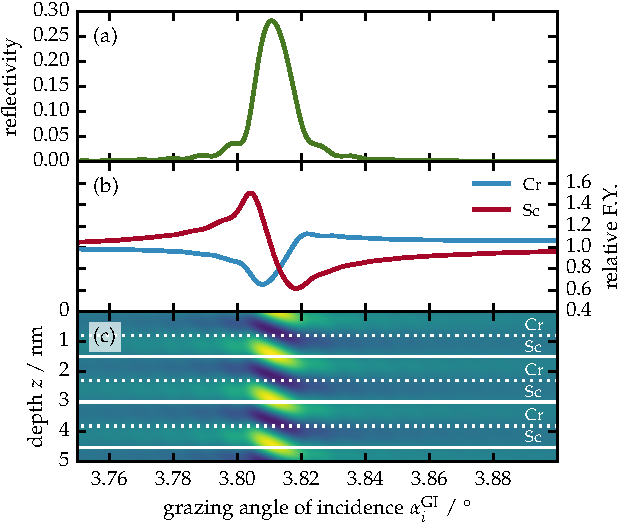
\includegraphics{img/XRF_scheme}
        \caption[X-ray standing wave fluorescence principle.]{%
            Illustration of the grazing incidence X-ray standing wave fluorescence analysis. The exemplary system shown is a bilayer multilayer mirror of Cr and Sc irradiated with a $6.25$ keV photon beam at grazing angles. Changing the grazing angle of incidence $\alpha_i^\text{GI}$ across the first Bragg peak (a) causes a standing wave inside the multilayer (total intensity in first top layers shown in (c)) and cause a relative fluorescence yield for the two different materials as shown in (b). The dotted lines in (a) and (b) indicate the case of interdiffusion and strongly asymmetric interface regions for comparison.}
        \label{ch_theo:fig_xrf_scheme}
\end{figure}

The constructive interference in the Bragg condition, in addition to resulting in a high reflectance, causes the formation of a X-ray standing wave inside the layers. The corresponding intensity distribution in the top first few layer pairs for the example given here is shown in Fig.~\ref{ch_theo:fig_xrf_scheme}(c). The standing wave intensity shifts through the individual layers thereby selectively exciting fluorescence radiation in the respective chemical species while changing the angle of incidence across the Bragg peak. Thus, this yields a method for chemically selective composition analysis with spatial resolution in the sub-nanometer regime called \gls{xsw} analysis. The response curves of the respective relative fluorescence radiation intensity across the Bragg peak for both materials is shown in Fig.~\ref{ch_theo:fig_xrf_scheme}(b). In this example, the fluorescence radiation was calculated according to the discrete sum in Eq.~\eqref{ch_theo:eqn_I_GIXRF_multilayer_discrete} with a sublayer setup as indicated in Fig.~\ref{ch_theo:fig_xrf_multilayer_scheme}(b) and $30$ sublayers per layer pair in each period.

We extended the example above to the case of imperfect layer stacks with interdiffusion and strongly asymmetric interface region thickness. The corresponding calculation is then calculated according to the scheme given in Fig.~\ref{ch_theo:fig_xrf_multilayer_scheme}(c) and is added for comparison to the reflectance and fluorescence yield curves in Fig.~\ref{ch_theo:fig_xrf_scheme}(a) and \ref{ch_theo:fig_xrf_scheme}(b) as dotted lines. The diminished contrast causes a decrease in the peak reflectance of that multilayer system as well as changes in the fluorescence yield.




    \chapter{Mo/Si Multilayer}

\section{Specular EUV reflectance}

\subsection{Reconstruction of the Layer Structure}

\section{Near-normal Incidence Diffuse Scattering}

\subsection{Kiessig-like Peaks and Resonant Effects}

\subsection{Tilted Bragg Sheets}

\subsection{Reconstruction of the PSD and the Multilayer Enhancement Factor}
    \chapter{Cr/Sc Multilayer}

\section{Layer setup}
\cite{haase_multiparameter_2016}
    \chapter{Higher-order Yoneda Effects on Lamellar Gratings}

    \chapter{Summary and Outlook} \label{ch_summary}
This thesis is dedicated to the characterization of multilayer mirrors systems by means of the combination of several indirect methods based on reflection, fluorescence and scattering using \gls{euv} and X-ray radiation. The systems investigated in this framework belong to two very important applications using wavelengths within the \gls{euv} range. With the semiconductor industry moving towards next-generation lithography systems employing radiation at \nm{13.5}, multilayer mirrors made from Mo/Si layers with the addition of different barrier layers were characterized with respect to their structure and interface morphology. The second system of interest in the presented study are suitable to reflect radiation in the water window spectral range. More specifically, for radiation close to the Sc L-edge at approximately \nm{3.1}. For that purpose, \gls{euv} reflectivity, \gls{xrr}, \gls{reuv} and \gls{xrf} have been applied as methods to determine the layer structure.

It has been demonstrated that the problem of uniqueness and accuracy associated with the structural reconstruction of such systems is of high relevance to deduct reliable reconstructions.
    %\include{pFundamentals}
    %\include{pExperimental}
    %\include{pNanometro}
    %\include{pPolymer}
    %\include{pXrr}
    \ifdraft{}{\pagestyle{thesisINTRO}}
    %\include{pSummary}

    %\ifdraft{}{\pagestyle{thesisINTRO}}
    \printbibliography[heading=bibintoc,title={References}]


\backmatter
    \pagestyle{thesisINTRO}
    \pagestyle{empty}
\selectlanguage{ngerman}
\noindent
\section*{Acknowledgement}
At this point, I would like to express my gratitude to all of those who directly or indirectly contributed to the successful completion of this thesis.

First and foremost, I would like to thank Dr.~Frank Scholze, head of the EUV radiometry group at the Physikalisch-Technische Bundesanstalt, for giving me the chance to conduct the work leading to this PhD thesis under his supervision. Our numerous scientific discussions, his valuable ideas and his constructive criticism bundled with the opportunity to conduct experiments even on a short notice, contributed significantly to the success of this thesis.

Furthermore, I would like to thank Prof.~Dr.~Mathias Richter for his support and the examination of this thesis. He always had an open ear and valuable advise for the course of my scientific work and the near future. 

I am very grateful to Prof.~Dr.~Stefan Eisebitt for supporting and evaluating my dissertation and to Dr.~Sa\v{s}a Bajt for the fruitful discussions and collaboration, for providing me with the Cr/Sc samples for my experiments and her willingness to serve as evaluator of this thesis. In addition, I thank Dr.~Stefan Braun for contributing the Mo/Si multilayer mirror samples.

I also like to acknowledge all of my current and former colleagues and fellow graduate students, first of all my mentor, Dr.~Victor Soltwisch, who supported me during the past years. I would also like to thank Anal\'{i}a Fern\'{a}ndez Herrero, Raül Garc\'{i}a Diez, Dr.~Christian Gollwitzer, Dr.~Philipp Hönicke, Mika Pflüger and Dr.~Jan Wernecke. Our many intense discussions and the collaborative atmosphere they helped to establish improved my research significantly.

I am sincerely grateful to all members of the working group 7.12, Christian Buchholz, Ayhan Babalik, Anja Babuschkin, Martin Biel, Benjamin Dubrau, Andreas Fischer, Anne Hesse, Sina Jaroslawzew, Florian Knorr, Dr.~Christian Laubis, Jana Lehnert, Heiko Mentzel, Jana Puls, Anja Schönstedt, Christian Stadelhoff. Without their support and patience in many late-night beamtimes in the laboratory, this work would not have been possible. My honest thanks also go to all other colleagues of the PTB in Berlin-Adlershof.

Finally, I am in dept to all of my friends and family for their endless support and their distractions during my studies and over the course of my PhD thesis. Most importantly I would like to name Michl, Michael, Paul, Laura, Tim, Anna, Leo and my parents Detlev and Martina. Last but not least, I am deeply grateful to my grandfather Dr.~Walther Neudert for inspiring me and his early encouragement of my scientific career.








\cleardoublepage

    \selectlanguage{ngerman}

\section*{Eidesstattliche Versicherung}
\vspace{3ex}

Hiermit versichere ich an Eides statt, dass ich die vorliegende Arbeit selbstständig verfasst und keine anderen als die in der Dissertation angegebenen Quellen und Hilfsmittel benutzt habe.
Alle Ausführungen, die anderen veröffentlichten oder nicht veröffentlichten Schriften wörtlich oder sinngemäß entnommen wurden, habe ich kenntlich gemacht.
Die Darstellung des Eigenanteils an bereits publizierten Inhalten in meiner beigefügten Erklärung ist zutreffend.
\vspace{3cm}

\noindent Berlin, den \today \hfill Anton Haase

\cleardoublepage

    %% publication list
\noindent
\pagestyle{empty}
\selectlanguage{ngerman}

\section*{Erklärung}

Es wurden bereits Teile der Dissertation veröffentlicht.
\vspace{2ex}

Liste der Veröffentlichungen, welche in die Dissertation eingeflossen sind:

\begin{enumerate}[label=\arabic*) ]
    \item \fullcite{haase_role_2014} 

    \item \fullcite{haase_characterization_2015} 

    \item \fullcite{haase_multiparameter_2016} 

    \item \fullcite{haase_interface_2017} 

\end{enumerate}
Liste der Veröffentlichungen, welche nicht in die Dissertation eingeflossen sind:
\begin{enumerate}[label=\arabic*) ]
    \item \fullcite{prasciolu_extended_2015} 

    \item \fullcite{soltwisch_correlated_2016} 
    
\end{enumerate}


Ich habe an keiner anderen Hochschule oder Fakultät eine Promotionsabsicht eingereicht.

\vspace{3cm}

\noindent Berlin, den \today \hfill Anton Haase

\cleardoublepage


    %\ifdraft{}{%
        %\printglossary[title=Glossary]
        %\printglossary[type=\acronymtype,title=Abbreviations,style=list]
        %\printglossary[type=symbols,title=Symbols,style=long,nonumberlist=true]
    %}

\end{document}
